\todo[inline,color=yellow]{Apresentar os resultados experimentais, inclua eventuais medidas de caracterização de componente (e.g., resistências, resistência parasítica do indutor). Avalie se é melhor apresentar o dado na forma de tabela ou gráfico. Note que um diagrama de Bode não deve ser apresentado na forma de tabela, enquanto que os valores de resistência utilizados poderiam utilizar este formato de apresentação.
}

\subsection{Nota}
	\todo[inline,color=yellow]{Caso apresente dados que serão usados para ajustar um modelo teórico, aproveite o espaço do gráfico para apresentar o ajuste. Faça uma breve discussão do ajuste,incluindo os parâmetros extraídos e equações utilizadas (evite deduções nesta parte). Sendo seu experimento constituído de mais de um conjunto de dados, utilize subseções.
}

\begin{figure}
	\centering
	% 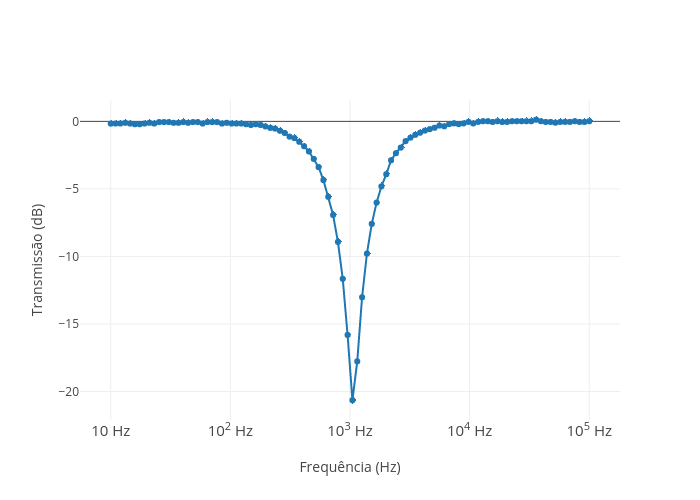
\includegraphics[width=0.9\textwidth]{figuras/diagrama-bode.png}
	%% Creator: Matplotlib, PGF backend
%%
%% To include the figure in your LaTeX document, write
%%   \input{<filename>.pgf}
%%
%% Make sure the required packages are loaded in your preamble
%%   \usepackage{pgf}
%%
%% Figures using additional raster images can only be included by \input if
%% they are in the same directory as the main LaTeX file. For loading figures
%% from other directories you can use the `import` package
%%   \usepackage{import}
%% and then include the figures with
%%   \import{<path to file>}{<filename>.pgf}
%%
%% Matplotlib used the following preamble
%%   \usepackage{fontspec}
%%   \setsansfont{DejaVu Sans}
%%   \setmonofont{DejaVu Sans Mono}
%%
\begingroup%
\makeatletter%
\begin{pgfpicture}%
\pgfpathrectangle{\pgfpointorigin}{\pgfqpoint{6.000000in}{4.000000in}}%
\pgfusepath{use as bounding box, clip}%
\begin{pgfscope}%
\pgfsetbuttcap%
\pgfsetmiterjoin%
\definecolor{currentfill}{rgb}{1.000000,1.000000,1.000000}%
\pgfsetfillcolor{currentfill}%
\pgfsetlinewidth{0.000000pt}%
\definecolor{currentstroke}{rgb}{1.000000,1.000000,1.000000}%
\pgfsetstrokecolor{currentstroke}%
\pgfsetdash{}{0pt}%
\pgfpathmoveto{\pgfqpoint{0.000000in}{0.000000in}}%
\pgfpathlineto{\pgfqpoint{6.000000in}{0.000000in}}%
\pgfpathlineto{\pgfqpoint{6.000000in}{4.000000in}}%
\pgfpathlineto{\pgfqpoint{0.000000in}{4.000000in}}%
\pgfpathclose%
\pgfusepath{fill}%
\end{pgfscope}%
\begin{pgfscope}%
\pgfsetbuttcap%
\pgfsetmiterjoin%
\definecolor{currentfill}{rgb}{0.898039,0.898039,0.898039}%
\pgfsetfillcolor{currentfill}%
\pgfsetlinewidth{0.000000pt}%
\definecolor{currentstroke}{rgb}{0.000000,0.000000,0.000000}%
\pgfsetstrokecolor{currentstroke}%
\pgfsetstrokeopacity{0.000000}%
\pgfsetdash{}{0pt}%
\pgfpathmoveto{\pgfqpoint{0.750000in}{2.147273in}}%
\pgfpathlineto{\pgfqpoint{5.400000in}{2.147273in}}%
\pgfpathlineto{\pgfqpoint{5.400000in}{3.520000in}}%
\pgfpathlineto{\pgfqpoint{0.750000in}{3.520000in}}%
\pgfpathclose%
\pgfusepath{fill}%
\end{pgfscope}%
\begin{pgfscope}%
\pgfpathrectangle{\pgfqpoint{0.750000in}{2.147273in}}{\pgfqpoint{4.650000in}{1.372727in}}%
\pgfusepath{clip}%
\pgfsetrectcap%
\pgfsetroundjoin%
\pgfsetlinewidth{0.803000pt}%
\definecolor{currentstroke}{rgb}{1.000000,1.000000,1.000000}%
\pgfsetstrokecolor{currentstroke}%
\pgfsetdash{}{0pt}%
\pgfpathmoveto{\pgfqpoint{0.961364in}{2.147273in}}%
\pgfpathlineto{\pgfqpoint{0.961364in}{3.520000in}}%
\pgfusepath{stroke}%
\end{pgfscope}%
\begin{pgfscope}%
\pgfsetbuttcap%
\pgfsetroundjoin%
\definecolor{currentfill}{rgb}{0.000000,0.000000,0.000000}%
\pgfsetfillcolor{currentfill}%
\pgfsetlinewidth{0.803000pt}%
\definecolor{currentstroke}{rgb}{0.000000,0.000000,0.000000}%
\pgfsetstrokecolor{currentstroke}%
\pgfsetdash{}{0pt}%
\pgfsys@defobject{currentmarker}{\pgfqpoint{0.000000in}{-0.048611in}}{\pgfqpoint{0.000000in}{0.000000in}}{%
\pgfpathmoveto{\pgfqpoint{0.000000in}{0.000000in}}%
\pgfpathlineto{\pgfqpoint{0.000000in}{-0.048611in}}%
\pgfusepath{stroke,fill}%
}%
\begin{pgfscope}%
\pgfsys@transformshift{0.961364in}{2.147273in}%
\pgfsys@useobject{currentmarker}{}%
\end{pgfscope}%
\end{pgfscope}%
\begin{pgfscope}%
\pgftext[x=0.961364in,y=2.050051in,,top]{\rmfamily\fontsize{10.000000}{12.000000}\selectfont \(\displaystyle 10^{1}\)}%
\end{pgfscope}%
\begin{pgfscope}%
\pgfpathrectangle{\pgfqpoint{0.750000in}{2.147273in}}{\pgfqpoint{4.650000in}{1.372727in}}%
\pgfusepath{clip}%
\pgfsetrectcap%
\pgfsetroundjoin%
\pgfsetlinewidth{0.803000pt}%
\definecolor{currentstroke}{rgb}{1.000000,1.000000,1.000000}%
\pgfsetstrokecolor{currentstroke}%
\pgfsetdash{}{0pt}%
\pgfpathmoveto{\pgfqpoint{2.018182in}{2.147273in}}%
\pgfpathlineto{\pgfqpoint{2.018182in}{3.520000in}}%
\pgfusepath{stroke}%
\end{pgfscope}%
\begin{pgfscope}%
\pgfsetbuttcap%
\pgfsetroundjoin%
\definecolor{currentfill}{rgb}{0.000000,0.000000,0.000000}%
\pgfsetfillcolor{currentfill}%
\pgfsetlinewidth{0.803000pt}%
\definecolor{currentstroke}{rgb}{0.000000,0.000000,0.000000}%
\pgfsetstrokecolor{currentstroke}%
\pgfsetdash{}{0pt}%
\pgfsys@defobject{currentmarker}{\pgfqpoint{0.000000in}{-0.048611in}}{\pgfqpoint{0.000000in}{0.000000in}}{%
\pgfpathmoveto{\pgfqpoint{0.000000in}{0.000000in}}%
\pgfpathlineto{\pgfqpoint{0.000000in}{-0.048611in}}%
\pgfusepath{stroke,fill}%
}%
\begin{pgfscope}%
\pgfsys@transformshift{2.018182in}{2.147273in}%
\pgfsys@useobject{currentmarker}{}%
\end{pgfscope}%
\end{pgfscope}%
\begin{pgfscope}%
\pgftext[x=2.018182in,y=2.050051in,,top]{\rmfamily\fontsize{10.000000}{12.000000}\selectfont \(\displaystyle 10^{2}\)}%
\end{pgfscope}%
\begin{pgfscope}%
\pgfpathrectangle{\pgfqpoint{0.750000in}{2.147273in}}{\pgfqpoint{4.650000in}{1.372727in}}%
\pgfusepath{clip}%
\pgfsetrectcap%
\pgfsetroundjoin%
\pgfsetlinewidth{0.803000pt}%
\definecolor{currentstroke}{rgb}{1.000000,1.000000,1.000000}%
\pgfsetstrokecolor{currentstroke}%
\pgfsetdash{}{0pt}%
\pgfpathmoveto{\pgfqpoint{3.075000in}{2.147273in}}%
\pgfpathlineto{\pgfqpoint{3.075000in}{3.520000in}}%
\pgfusepath{stroke}%
\end{pgfscope}%
\begin{pgfscope}%
\pgfsetbuttcap%
\pgfsetroundjoin%
\definecolor{currentfill}{rgb}{0.000000,0.000000,0.000000}%
\pgfsetfillcolor{currentfill}%
\pgfsetlinewidth{0.803000pt}%
\definecolor{currentstroke}{rgb}{0.000000,0.000000,0.000000}%
\pgfsetstrokecolor{currentstroke}%
\pgfsetdash{}{0pt}%
\pgfsys@defobject{currentmarker}{\pgfqpoint{0.000000in}{-0.048611in}}{\pgfqpoint{0.000000in}{0.000000in}}{%
\pgfpathmoveto{\pgfqpoint{0.000000in}{0.000000in}}%
\pgfpathlineto{\pgfqpoint{0.000000in}{-0.048611in}}%
\pgfusepath{stroke,fill}%
}%
\begin{pgfscope}%
\pgfsys@transformshift{3.075000in}{2.147273in}%
\pgfsys@useobject{currentmarker}{}%
\end{pgfscope}%
\end{pgfscope}%
\begin{pgfscope}%
\pgftext[x=3.075000in,y=2.050051in,,top]{\rmfamily\fontsize{10.000000}{12.000000}\selectfont \(\displaystyle 10^{3}\)}%
\end{pgfscope}%
\begin{pgfscope}%
\pgfpathrectangle{\pgfqpoint{0.750000in}{2.147273in}}{\pgfqpoint{4.650000in}{1.372727in}}%
\pgfusepath{clip}%
\pgfsetrectcap%
\pgfsetroundjoin%
\pgfsetlinewidth{0.803000pt}%
\definecolor{currentstroke}{rgb}{1.000000,1.000000,1.000000}%
\pgfsetstrokecolor{currentstroke}%
\pgfsetdash{}{0pt}%
\pgfpathmoveto{\pgfqpoint{4.131818in}{2.147273in}}%
\pgfpathlineto{\pgfqpoint{4.131818in}{3.520000in}}%
\pgfusepath{stroke}%
\end{pgfscope}%
\begin{pgfscope}%
\pgfsetbuttcap%
\pgfsetroundjoin%
\definecolor{currentfill}{rgb}{0.000000,0.000000,0.000000}%
\pgfsetfillcolor{currentfill}%
\pgfsetlinewidth{0.803000pt}%
\definecolor{currentstroke}{rgb}{0.000000,0.000000,0.000000}%
\pgfsetstrokecolor{currentstroke}%
\pgfsetdash{}{0pt}%
\pgfsys@defobject{currentmarker}{\pgfqpoint{0.000000in}{-0.048611in}}{\pgfqpoint{0.000000in}{0.000000in}}{%
\pgfpathmoveto{\pgfqpoint{0.000000in}{0.000000in}}%
\pgfpathlineto{\pgfqpoint{0.000000in}{-0.048611in}}%
\pgfusepath{stroke,fill}%
}%
\begin{pgfscope}%
\pgfsys@transformshift{4.131818in}{2.147273in}%
\pgfsys@useobject{currentmarker}{}%
\end{pgfscope}%
\end{pgfscope}%
\begin{pgfscope}%
\pgftext[x=4.131818in,y=2.050051in,,top]{\rmfamily\fontsize{10.000000}{12.000000}\selectfont \(\displaystyle 10^{4}\)}%
\end{pgfscope}%
\begin{pgfscope}%
\pgfpathrectangle{\pgfqpoint{0.750000in}{2.147273in}}{\pgfqpoint{4.650000in}{1.372727in}}%
\pgfusepath{clip}%
\pgfsetrectcap%
\pgfsetroundjoin%
\pgfsetlinewidth{0.803000pt}%
\definecolor{currentstroke}{rgb}{1.000000,1.000000,1.000000}%
\pgfsetstrokecolor{currentstroke}%
\pgfsetdash{}{0pt}%
\pgfpathmoveto{\pgfqpoint{5.188636in}{2.147273in}}%
\pgfpathlineto{\pgfqpoint{5.188636in}{3.520000in}}%
\pgfusepath{stroke}%
\end{pgfscope}%
\begin{pgfscope}%
\pgfsetbuttcap%
\pgfsetroundjoin%
\definecolor{currentfill}{rgb}{0.000000,0.000000,0.000000}%
\pgfsetfillcolor{currentfill}%
\pgfsetlinewidth{0.803000pt}%
\definecolor{currentstroke}{rgb}{0.000000,0.000000,0.000000}%
\pgfsetstrokecolor{currentstroke}%
\pgfsetdash{}{0pt}%
\pgfsys@defobject{currentmarker}{\pgfqpoint{0.000000in}{-0.048611in}}{\pgfqpoint{0.000000in}{0.000000in}}{%
\pgfpathmoveto{\pgfqpoint{0.000000in}{0.000000in}}%
\pgfpathlineto{\pgfqpoint{0.000000in}{-0.048611in}}%
\pgfusepath{stroke,fill}%
}%
\begin{pgfscope}%
\pgfsys@transformshift{5.188636in}{2.147273in}%
\pgfsys@useobject{currentmarker}{}%
\end{pgfscope}%
\end{pgfscope}%
\begin{pgfscope}%
\pgftext[x=5.188636in,y=2.050051in,,top]{\rmfamily\fontsize{10.000000}{12.000000}\selectfont \(\displaystyle 10^{5}\)}%
\end{pgfscope}%
\begin{pgfscope}%
\pgfsetbuttcap%
\pgfsetroundjoin%
\definecolor{currentfill}{rgb}{0.000000,0.000000,0.000000}%
\pgfsetfillcolor{currentfill}%
\pgfsetlinewidth{0.602250pt}%
\definecolor{currentstroke}{rgb}{0.000000,0.000000,0.000000}%
\pgfsetstrokecolor{currentstroke}%
\pgfsetdash{}{0pt}%
\pgfsys@defobject{currentmarker}{\pgfqpoint{0.000000in}{-0.027778in}}{\pgfqpoint{0.000000in}{0.000000in}}{%
\pgfpathmoveto{\pgfqpoint{0.000000in}{0.000000in}}%
\pgfpathlineto{\pgfqpoint{0.000000in}{-0.027778in}}%
\pgfusepath{stroke,fill}%
}%
\begin{pgfscope}%
\pgfsys@transformshift{0.797660in}{2.147273in}%
\pgfsys@useobject{currentmarker}{}%
\end{pgfscope}%
\end{pgfscope}%
\begin{pgfscope}%
\pgfsetbuttcap%
\pgfsetroundjoin%
\definecolor{currentfill}{rgb}{0.000000,0.000000,0.000000}%
\pgfsetfillcolor{currentfill}%
\pgfsetlinewidth{0.602250pt}%
\definecolor{currentstroke}{rgb}{0.000000,0.000000,0.000000}%
\pgfsetstrokecolor{currentstroke}%
\pgfsetdash{}{0pt}%
\pgfsys@defobject{currentmarker}{\pgfqpoint{0.000000in}{-0.027778in}}{\pgfqpoint{0.000000in}{0.000000in}}{%
\pgfpathmoveto{\pgfqpoint{0.000000in}{0.000000in}}%
\pgfpathlineto{\pgfqpoint{0.000000in}{-0.027778in}}%
\pgfusepath{stroke,fill}%
}%
\begin{pgfscope}%
\pgfsys@transformshift{0.858947in}{2.147273in}%
\pgfsys@useobject{currentmarker}{}%
\end{pgfscope}%
\end{pgfscope}%
\begin{pgfscope}%
\pgfsetbuttcap%
\pgfsetroundjoin%
\definecolor{currentfill}{rgb}{0.000000,0.000000,0.000000}%
\pgfsetfillcolor{currentfill}%
\pgfsetlinewidth{0.602250pt}%
\definecolor{currentstroke}{rgb}{0.000000,0.000000,0.000000}%
\pgfsetstrokecolor{currentstroke}%
\pgfsetdash{}{0pt}%
\pgfsys@defobject{currentmarker}{\pgfqpoint{0.000000in}{-0.027778in}}{\pgfqpoint{0.000000in}{0.000000in}}{%
\pgfpathmoveto{\pgfqpoint{0.000000in}{0.000000in}}%
\pgfpathlineto{\pgfqpoint{0.000000in}{-0.027778in}}%
\pgfusepath{stroke,fill}%
}%
\begin{pgfscope}%
\pgfsys@transformshift{0.913006in}{2.147273in}%
\pgfsys@useobject{currentmarker}{}%
\end{pgfscope}%
\end{pgfscope}%
\begin{pgfscope}%
\pgfsetbuttcap%
\pgfsetroundjoin%
\definecolor{currentfill}{rgb}{0.000000,0.000000,0.000000}%
\pgfsetfillcolor{currentfill}%
\pgfsetlinewidth{0.602250pt}%
\definecolor{currentstroke}{rgb}{0.000000,0.000000,0.000000}%
\pgfsetstrokecolor{currentstroke}%
\pgfsetdash{}{0pt}%
\pgfsys@defobject{currentmarker}{\pgfqpoint{0.000000in}{-0.027778in}}{\pgfqpoint{0.000000in}{0.000000in}}{%
\pgfpathmoveto{\pgfqpoint{0.000000in}{0.000000in}}%
\pgfpathlineto{\pgfqpoint{0.000000in}{-0.027778in}}%
\pgfusepath{stroke,fill}%
}%
\begin{pgfscope}%
\pgfsys@transformshift{1.279498in}{2.147273in}%
\pgfsys@useobject{currentmarker}{}%
\end{pgfscope}%
\end{pgfscope}%
\begin{pgfscope}%
\pgfsetbuttcap%
\pgfsetroundjoin%
\definecolor{currentfill}{rgb}{0.000000,0.000000,0.000000}%
\pgfsetfillcolor{currentfill}%
\pgfsetlinewidth{0.602250pt}%
\definecolor{currentstroke}{rgb}{0.000000,0.000000,0.000000}%
\pgfsetstrokecolor{currentstroke}%
\pgfsetdash{}{0pt}%
\pgfsys@defobject{currentmarker}{\pgfqpoint{0.000000in}{-0.027778in}}{\pgfqpoint{0.000000in}{0.000000in}}{%
\pgfpathmoveto{\pgfqpoint{0.000000in}{0.000000in}}%
\pgfpathlineto{\pgfqpoint{0.000000in}{-0.027778in}}%
\pgfusepath{stroke,fill}%
}%
\begin{pgfscope}%
\pgfsys@transformshift{1.465594in}{2.147273in}%
\pgfsys@useobject{currentmarker}{}%
\end{pgfscope}%
\end{pgfscope}%
\begin{pgfscope}%
\pgfsetbuttcap%
\pgfsetroundjoin%
\definecolor{currentfill}{rgb}{0.000000,0.000000,0.000000}%
\pgfsetfillcolor{currentfill}%
\pgfsetlinewidth{0.602250pt}%
\definecolor{currentstroke}{rgb}{0.000000,0.000000,0.000000}%
\pgfsetstrokecolor{currentstroke}%
\pgfsetdash{}{0pt}%
\pgfsys@defobject{currentmarker}{\pgfqpoint{0.000000in}{-0.027778in}}{\pgfqpoint{0.000000in}{0.000000in}}{%
\pgfpathmoveto{\pgfqpoint{0.000000in}{0.000000in}}%
\pgfpathlineto{\pgfqpoint{0.000000in}{-0.027778in}}%
\pgfusepath{stroke,fill}%
}%
\begin{pgfscope}%
\pgfsys@transformshift{1.597632in}{2.147273in}%
\pgfsys@useobject{currentmarker}{}%
\end{pgfscope}%
\end{pgfscope}%
\begin{pgfscope}%
\pgfsetbuttcap%
\pgfsetroundjoin%
\definecolor{currentfill}{rgb}{0.000000,0.000000,0.000000}%
\pgfsetfillcolor{currentfill}%
\pgfsetlinewidth{0.602250pt}%
\definecolor{currentstroke}{rgb}{0.000000,0.000000,0.000000}%
\pgfsetstrokecolor{currentstroke}%
\pgfsetdash{}{0pt}%
\pgfsys@defobject{currentmarker}{\pgfqpoint{0.000000in}{-0.027778in}}{\pgfqpoint{0.000000in}{0.000000in}}{%
\pgfpathmoveto{\pgfqpoint{0.000000in}{0.000000in}}%
\pgfpathlineto{\pgfqpoint{0.000000in}{-0.027778in}}%
\pgfusepath{stroke,fill}%
}%
\begin{pgfscope}%
\pgfsys@transformshift{1.700048in}{2.147273in}%
\pgfsys@useobject{currentmarker}{}%
\end{pgfscope}%
\end{pgfscope}%
\begin{pgfscope}%
\pgfsetbuttcap%
\pgfsetroundjoin%
\definecolor{currentfill}{rgb}{0.000000,0.000000,0.000000}%
\pgfsetfillcolor{currentfill}%
\pgfsetlinewidth{0.602250pt}%
\definecolor{currentstroke}{rgb}{0.000000,0.000000,0.000000}%
\pgfsetstrokecolor{currentstroke}%
\pgfsetdash{}{0pt}%
\pgfsys@defobject{currentmarker}{\pgfqpoint{0.000000in}{-0.027778in}}{\pgfqpoint{0.000000in}{0.000000in}}{%
\pgfpathmoveto{\pgfqpoint{0.000000in}{0.000000in}}%
\pgfpathlineto{\pgfqpoint{0.000000in}{-0.027778in}}%
\pgfusepath{stroke,fill}%
}%
\begin{pgfscope}%
\pgfsys@transformshift{1.783728in}{2.147273in}%
\pgfsys@useobject{currentmarker}{}%
\end{pgfscope}%
\end{pgfscope}%
\begin{pgfscope}%
\pgfsetbuttcap%
\pgfsetroundjoin%
\definecolor{currentfill}{rgb}{0.000000,0.000000,0.000000}%
\pgfsetfillcolor{currentfill}%
\pgfsetlinewidth{0.602250pt}%
\definecolor{currentstroke}{rgb}{0.000000,0.000000,0.000000}%
\pgfsetstrokecolor{currentstroke}%
\pgfsetdash{}{0pt}%
\pgfsys@defobject{currentmarker}{\pgfqpoint{0.000000in}{-0.027778in}}{\pgfqpoint{0.000000in}{0.000000in}}{%
\pgfpathmoveto{\pgfqpoint{0.000000in}{0.000000in}}%
\pgfpathlineto{\pgfqpoint{0.000000in}{-0.027778in}}%
\pgfusepath{stroke,fill}%
}%
\begin{pgfscope}%
\pgfsys@transformshift{1.854479in}{2.147273in}%
\pgfsys@useobject{currentmarker}{}%
\end{pgfscope}%
\end{pgfscope}%
\begin{pgfscope}%
\pgfsetbuttcap%
\pgfsetroundjoin%
\definecolor{currentfill}{rgb}{0.000000,0.000000,0.000000}%
\pgfsetfillcolor{currentfill}%
\pgfsetlinewidth{0.602250pt}%
\definecolor{currentstroke}{rgb}{0.000000,0.000000,0.000000}%
\pgfsetstrokecolor{currentstroke}%
\pgfsetdash{}{0pt}%
\pgfsys@defobject{currentmarker}{\pgfqpoint{0.000000in}{-0.027778in}}{\pgfqpoint{0.000000in}{0.000000in}}{%
\pgfpathmoveto{\pgfqpoint{0.000000in}{0.000000in}}%
\pgfpathlineto{\pgfqpoint{0.000000in}{-0.027778in}}%
\pgfusepath{stroke,fill}%
}%
\begin{pgfscope}%
\pgfsys@transformshift{1.915766in}{2.147273in}%
\pgfsys@useobject{currentmarker}{}%
\end{pgfscope}%
\end{pgfscope}%
\begin{pgfscope}%
\pgfsetbuttcap%
\pgfsetroundjoin%
\definecolor{currentfill}{rgb}{0.000000,0.000000,0.000000}%
\pgfsetfillcolor{currentfill}%
\pgfsetlinewidth{0.602250pt}%
\definecolor{currentstroke}{rgb}{0.000000,0.000000,0.000000}%
\pgfsetstrokecolor{currentstroke}%
\pgfsetdash{}{0pt}%
\pgfsys@defobject{currentmarker}{\pgfqpoint{0.000000in}{-0.027778in}}{\pgfqpoint{0.000000in}{0.000000in}}{%
\pgfpathmoveto{\pgfqpoint{0.000000in}{0.000000in}}%
\pgfpathlineto{\pgfqpoint{0.000000in}{-0.027778in}}%
\pgfusepath{stroke,fill}%
}%
\begin{pgfscope}%
\pgfsys@transformshift{1.969824in}{2.147273in}%
\pgfsys@useobject{currentmarker}{}%
\end{pgfscope}%
\end{pgfscope}%
\begin{pgfscope}%
\pgfsetbuttcap%
\pgfsetroundjoin%
\definecolor{currentfill}{rgb}{0.000000,0.000000,0.000000}%
\pgfsetfillcolor{currentfill}%
\pgfsetlinewidth{0.602250pt}%
\definecolor{currentstroke}{rgb}{0.000000,0.000000,0.000000}%
\pgfsetstrokecolor{currentstroke}%
\pgfsetdash{}{0pt}%
\pgfsys@defobject{currentmarker}{\pgfqpoint{0.000000in}{-0.027778in}}{\pgfqpoint{0.000000in}{0.000000in}}{%
\pgfpathmoveto{\pgfqpoint{0.000000in}{0.000000in}}%
\pgfpathlineto{\pgfqpoint{0.000000in}{-0.027778in}}%
\pgfusepath{stroke,fill}%
}%
\begin{pgfscope}%
\pgfsys@transformshift{2.336316in}{2.147273in}%
\pgfsys@useobject{currentmarker}{}%
\end{pgfscope}%
\end{pgfscope}%
\begin{pgfscope}%
\pgfsetbuttcap%
\pgfsetroundjoin%
\definecolor{currentfill}{rgb}{0.000000,0.000000,0.000000}%
\pgfsetfillcolor{currentfill}%
\pgfsetlinewidth{0.602250pt}%
\definecolor{currentstroke}{rgb}{0.000000,0.000000,0.000000}%
\pgfsetstrokecolor{currentstroke}%
\pgfsetdash{}{0pt}%
\pgfsys@defobject{currentmarker}{\pgfqpoint{0.000000in}{-0.027778in}}{\pgfqpoint{0.000000in}{0.000000in}}{%
\pgfpathmoveto{\pgfqpoint{0.000000in}{0.000000in}}%
\pgfpathlineto{\pgfqpoint{0.000000in}{-0.027778in}}%
\pgfusepath{stroke,fill}%
}%
\begin{pgfscope}%
\pgfsys@transformshift{2.522412in}{2.147273in}%
\pgfsys@useobject{currentmarker}{}%
\end{pgfscope}%
\end{pgfscope}%
\begin{pgfscope}%
\pgfsetbuttcap%
\pgfsetroundjoin%
\definecolor{currentfill}{rgb}{0.000000,0.000000,0.000000}%
\pgfsetfillcolor{currentfill}%
\pgfsetlinewidth{0.602250pt}%
\definecolor{currentstroke}{rgb}{0.000000,0.000000,0.000000}%
\pgfsetstrokecolor{currentstroke}%
\pgfsetdash{}{0pt}%
\pgfsys@defobject{currentmarker}{\pgfqpoint{0.000000in}{-0.027778in}}{\pgfqpoint{0.000000in}{0.000000in}}{%
\pgfpathmoveto{\pgfqpoint{0.000000in}{0.000000in}}%
\pgfpathlineto{\pgfqpoint{0.000000in}{-0.027778in}}%
\pgfusepath{stroke,fill}%
}%
\begin{pgfscope}%
\pgfsys@transformshift{2.654450in}{2.147273in}%
\pgfsys@useobject{currentmarker}{}%
\end{pgfscope}%
\end{pgfscope}%
\begin{pgfscope}%
\pgfsetbuttcap%
\pgfsetroundjoin%
\definecolor{currentfill}{rgb}{0.000000,0.000000,0.000000}%
\pgfsetfillcolor{currentfill}%
\pgfsetlinewidth{0.602250pt}%
\definecolor{currentstroke}{rgb}{0.000000,0.000000,0.000000}%
\pgfsetstrokecolor{currentstroke}%
\pgfsetdash{}{0pt}%
\pgfsys@defobject{currentmarker}{\pgfqpoint{0.000000in}{-0.027778in}}{\pgfqpoint{0.000000in}{0.000000in}}{%
\pgfpathmoveto{\pgfqpoint{0.000000in}{0.000000in}}%
\pgfpathlineto{\pgfqpoint{0.000000in}{-0.027778in}}%
\pgfusepath{stroke,fill}%
}%
\begin{pgfscope}%
\pgfsys@transformshift{2.756866in}{2.147273in}%
\pgfsys@useobject{currentmarker}{}%
\end{pgfscope}%
\end{pgfscope}%
\begin{pgfscope}%
\pgfsetbuttcap%
\pgfsetroundjoin%
\definecolor{currentfill}{rgb}{0.000000,0.000000,0.000000}%
\pgfsetfillcolor{currentfill}%
\pgfsetlinewidth{0.602250pt}%
\definecolor{currentstroke}{rgb}{0.000000,0.000000,0.000000}%
\pgfsetstrokecolor{currentstroke}%
\pgfsetdash{}{0pt}%
\pgfsys@defobject{currentmarker}{\pgfqpoint{0.000000in}{-0.027778in}}{\pgfqpoint{0.000000in}{0.000000in}}{%
\pgfpathmoveto{\pgfqpoint{0.000000in}{0.000000in}}%
\pgfpathlineto{\pgfqpoint{0.000000in}{-0.027778in}}%
\pgfusepath{stroke,fill}%
}%
\begin{pgfscope}%
\pgfsys@transformshift{2.840546in}{2.147273in}%
\pgfsys@useobject{currentmarker}{}%
\end{pgfscope}%
\end{pgfscope}%
\begin{pgfscope}%
\pgfsetbuttcap%
\pgfsetroundjoin%
\definecolor{currentfill}{rgb}{0.000000,0.000000,0.000000}%
\pgfsetfillcolor{currentfill}%
\pgfsetlinewidth{0.602250pt}%
\definecolor{currentstroke}{rgb}{0.000000,0.000000,0.000000}%
\pgfsetstrokecolor{currentstroke}%
\pgfsetdash{}{0pt}%
\pgfsys@defobject{currentmarker}{\pgfqpoint{0.000000in}{-0.027778in}}{\pgfqpoint{0.000000in}{0.000000in}}{%
\pgfpathmoveto{\pgfqpoint{0.000000in}{0.000000in}}%
\pgfpathlineto{\pgfqpoint{0.000000in}{-0.027778in}}%
\pgfusepath{stroke,fill}%
}%
\begin{pgfscope}%
\pgfsys@transformshift{2.911297in}{2.147273in}%
\pgfsys@useobject{currentmarker}{}%
\end{pgfscope}%
\end{pgfscope}%
\begin{pgfscope}%
\pgfsetbuttcap%
\pgfsetroundjoin%
\definecolor{currentfill}{rgb}{0.000000,0.000000,0.000000}%
\pgfsetfillcolor{currentfill}%
\pgfsetlinewidth{0.602250pt}%
\definecolor{currentstroke}{rgb}{0.000000,0.000000,0.000000}%
\pgfsetstrokecolor{currentstroke}%
\pgfsetdash{}{0pt}%
\pgfsys@defobject{currentmarker}{\pgfqpoint{0.000000in}{-0.027778in}}{\pgfqpoint{0.000000in}{0.000000in}}{%
\pgfpathmoveto{\pgfqpoint{0.000000in}{0.000000in}}%
\pgfpathlineto{\pgfqpoint{0.000000in}{-0.027778in}}%
\pgfusepath{stroke,fill}%
}%
\begin{pgfscope}%
\pgfsys@transformshift{2.972584in}{2.147273in}%
\pgfsys@useobject{currentmarker}{}%
\end{pgfscope}%
\end{pgfscope}%
\begin{pgfscope}%
\pgfsetbuttcap%
\pgfsetroundjoin%
\definecolor{currentfill}{rgb}{0.000000,0.000000,0.000000}%
\pgfsetfillcolor{currentfill}%
\pgfsetlinewidth{0.602250pt}%
\definecolor{currentstroke}{rgb}{0.000000,0.000000,0.000000}%
\pgfsetstrokecolor{currentstroke}%
\pgfsetdash{}{0pt}%
\pgfsys@defobject{currentmarker}{\pgfqpoint{0.000000in}{-0.027778in}}{\pgfqpoint{0.000000in}{0.000000in}}{%
\pgfpathmoveto{\pgfqpoint{0.000000in}{0.000000in}}%
\pgfpathlineto{\pgfqpoint{0.000000in}{-0.027778in}}%
\pgfusepath{stroke,fill}%
}%
\begin{pgfscope}%
\pgfsys@transformshift{3.026643in}{2.147273in}%
\pgfsys@useobject{currentmarker}{}%
\end{pgfscope}%
\end{pgfscope}%
\begin{pgfscope}%
\pgfsetbuttcap%
\pgfsetroundjoin%
\definecolor{currentfill}{rgb}{0.000000,0.000000,0.000000}%
\pgfsetfillcolor{currentfill}%
\pgfsetlinewidth{0.602250pt}%
\definecolor{currentstroke}{rgb}{0.000000,0.000000,0.000000}%
\pgfsetstrokecolor{currentstroke}%
\pgfsetdash{}{0pt}%
\pgfsys@defobject{currentmarker}{\pgfqpoint{0.000000in}{-0.027778in}}{\pgfqpoint{0.000000in}{0.000000in}}{%
\pgfpathmoveto{\pgfqpoint{0.000000in}{0.000000in}}%
\pgfpathlineto{\pgfqpoint{0.000000in}{-0.027778in}}%
\pgfusepath{stroke,fill}%
}%
\begin{pgfscope}%
\pgfsys@transformshift{3.393134in}{2.147273in}%
\pgfsys@useobject{currentmarker}{}%
\end{pgfscope}%
\end{pgfscope}%
\begin{pgfscope}%
\pgfsetbuttcap%
\pgfsetroundjoin%
\definecolor{currentfill}{rgb}{0.000000,0.000000,0.000000}%
\pgfsetfillcolor{currentfill}%
\pgfsetlinewidth{0.602250pt}%
\definecolor{currentstroke}{rgb}{0.000000,0.000000,0.000000}%
\pgfsetstrokecolor{currentstroke}%
\pgfsetdash{}{0pt}%
\pgfsys@defobject{currentmarker}{\pgfqpoint{0.000000in}{-0.027778in}}{\pgfqpoint{0.000000in}{0.000000in}}{%
\pgfpathmoveto{\pgfqpoint{0.000000in}{0.000000in}}%
\pgfpathlineto{\pgfqpoint{0.000000in}{-0.027778in}}%
\pgfusepath{stroke,fill}%
}%
\begin{pgfscope}%
\pgfsys@transformshift{3.579230in}{2.147273in}%
\pgfsys@useobject{currentmarker}{}%
\end{pgfscope}%
\end{pgfscope}%
\begin{pgfscope}%
\pgfsetbuttcap%
\pgfsetroundjoin%
\definecolor{currentfill}{rgb}{0.000000,0.000000,0.000000}%
\pgfsetfillcolor{currentfill}%
\pgfsetlinewidth{0.602250pt}%
\definecolor{currentstroke}{rgb}{0.000000,0.000000,0.000000}%
\pgfsetstrokecolor{currentstroke}%
\pgfsetdash{}{0pt}%
\pgfsys@defobject{currentmarker}{\pgfqpoint{0.000000in}{-0.027778in}}{\pgfqpoint{0.000000in}{0.000000in}}{%
\pgfpathmoveto{\pgfqpoint{0.000000in}{0.000000in}}%
\pgfpathlineto{\pgfqpoint{0.000000in}{-0.027778in}}%
\pgfusepath{stroke,fill}%
}%
\begin{pgfscope}%
\pgfsys@transformshift{3.711268in}{2.147273in}%
\pgfsys@useobject{currentmarker}{}%
\end{pgfscope}%
\end{pgfscope}%
\begin{pgfscope}%
\pgfsetbuttcap%
\pgfsetroundjoin%
\definecolor{currentfill}{rgb}{0.000000,0.000000,0.000000}%
\pgfsetfillcolor{currentfill}%
\pgfsetlinewidth{0.602250pt}%
\definecolor{currentstroke}{rgb}{0.000000,0.000000,0.000000}%
\pgfsetstrokecolor{currentstroke}%
\pgfsetdash{}{0pt}%
\pgfsys@defobject{currentmarker}{\pgfqpoint{0.000000in}{-0.027778in}}{\pgfqpoint{0.000000in}{0.000000in}}{%
\pgfpathmoveto{\pgfqpoint{0.000000in}{0.000000in}}%
\pgfpathlineto{\pgfqpoint{0.000000in}{-0.027778in}}%
\pgfusepath{stroke,fill}%
}%
\begin{pgfscope}%
\pgfsys@transformshift{3.813684in}{2.147273in}%
\pgfsys@useobject{currentmarker}{}%
\end{pgfscope}%
\end{pgfscope}%
\begin{pgfscope}%
\pgfsetbuttcap%
\pgfsetroundjoin%
\definecolor{currentfill}{rgb}{0.000000,0.000000,0.000000}%
\pgfsetfillcolor{currentfill}%
\pgfsetlinewidth{0.602250pt}%
\definecolor{currentstroke}{rgb}{0.000000,0.000000,0.000000}%
\pgfsetstrokecolor{currentstroke}%
\pgfsetdash{}{0pt}%
\pgfsys@defobject{currentmarker}{\pgfqpoint{0.000000in}{-0.027778in}}{\pgfqpoint{0.000000in}{0.000000in}}{%
\pgfpathmoveto{\pgfqpoint{0.000000in}{0.000000in}}%
\pgfpathlineto{\pgfqpoint{0.000000in}{-0.027778in}}%
\pgfusepath{stroke,fill}%
}%
\begin{pgfscope}%
\pgfsys@transformshift{3.897364in}{2.147273in}%
\pgfsys@useobject{currentmarker}{}%
\end{pgfscope}%
\end{pgfscope}%
\begin{pgfscope}%
\pgfsetbuttcap%
\pgfsetroundjoin%
\definecolor{currentfill}{rgb}{0.000000,0.000000,0.000000}%
\pgfsetfillcolor{currentfill}%
\pgfsetlinewidth{0.602250pt}%
\definecolor{currentstroke}{rgb}{0.000000,0.000000,0.000000}%
\pgfsetstrokecolor{currentstroke}%
\pgfsetdash{}{0pt}%
\pgfsys@defobject{currentmarker}{\pgfqpoint{0.000000in}{-0.027778in}}{\pgfqpoint{0.000000in}{0.000000in}}{%
\pgfpathmoveto{\pgfqpoint{0.000000in}{0.000000in}}%
\pgfpathlineto{\pgfqpoint{0.000000in}{-0.027778in}}%
\pgfusepath{stroke,fill}%
}%
\begin{pgfscope}%
\pgfsys@transformshift{3.968115in}{2.147273in}%
\pgfsys@useobject{currentmarker}{}%
\end{pgfscope}%
\end{pgfscope}%
\begin{pgfscope}%
\pgfsetbuttcap%
\pgfsetroundjoin%
\definecolor{currentfill}{rgb}{0.000000,0.000000,0.000000}%
\pgfsetfillcolor{currentfill}%
\pgfsetlinewidth{0.602250pt}%
\definecolor{currentstroke}{rgb}{0.000000,0.000000,0.000000}%
\pgfsetstrokecolor{currentstroke}%
\pgfsetdash{}{0pt}%
\pgfsys@defobject{currentmarker}{\pgfqpoint{0.000000in}{-0.027778in}}{\pgfqpoint{0.000000in}{0.000000in}}{%
\pgfpathmoveto{\pgfqpoint{0.000000in}{0.000000in}}%
\pgfpathlineto{\pgfqpoint{0.000000in}{-0.027778in}}%
\pgfusepath{stroke,fill}%
}%
\begin{pgfscope}%
\pgfsys@transformshift{4.029402in}{2.147273in}%
\pgfsys@useobject{currentmarker}{}%
\end{pgfscope}%
\end{pgfscope}%
\begin{pgfscope}%
\pgfsetbuttcap%
\pgfsetroundjoin%
\definecolor{currentfill}{rgb}{0.000000,0.000000,0.000000}%
\pgfsetfillcolor{currentfill}%
\pgfsetlinewidth{0.602250pt}%
\definecolor{currentstroke}{rgb}{0.000000,0.000000,0.000000}%
\pgfsetstrokecolor{currentstroke}%
\pgfsetdash{}{0pt}%
\pgfsys@defobject{currentmarker}{\pgfqpoint{0.000000in}{-0.027778in}}{\pgfqpoint{0.000000in}{0.000000in}}{%
\pgfpathmoveto{\pgfqpoint{0.000000in}{0.000000in}}%
\pgfpathlineto{\pgfqpoint{0.000000in}{-0.027778in}}%
\pgfusepath{stroke,fill}%
}%
\begin{pgfscope}%
\pgfsys@transformshift{4.083461in}{2.147273in}%
\pgfsys@useobject{currentmarker}{}%
\end{pgfscope}%
\end{pgfscope}%
\begin{pgfscope}%
\pgfsetbuttcap%
\pgfsetroundjoin%
\definecolor{currentfill}{rgb}{0.000000,0.000000,0.000000}%
\pgfsetfillcolor{currentfill}%
\pgfsetlinewidth{0.602250pt}%
\definecolor{currentstroke}{rgb}{0.000000,0.000000,0.000000}%
\pgfsetstrokecolor{currentstroke}%
\pgfsetdash{}{0pt}%
\pgfsys@defobject{currentmarker}{\pgfqpoint{0.000000in}{-0.027778in}}{\pgfqpoint{0.000000in}{0.000000in}}{%
\pgfpathmoveto{\pgfqpoint{0.000000in}{0.000000in}}%
\pgfpathlineto{\pgfqpoint{0.000000in}{-0.027778in}}%
\pgfusepath{stroke,fill}%
}%
\begin{pgfscope}%
\pgfsys@transformshift{4.449952in}{2.147273in}%
\pgfsys@useobject{currentmarker}{}%
\end{pgfscope}%
\end{pgfscope}%
\begin{pgfscope}%
\pgfsetbuttcap%
\pgfsetroundjoin%
\definecolor{currentfill}{rgb}{0.000000,0.000000,0.000000}%
\pgfsetfillcolor{currentfill}%
\pgfsetlinewidth{0.602250pt}%
\definecolor{currentstroke}{rgb}{0.000000,0.000000,0.000000}%
\pgfsetstrokecolor{currentstroke}%
\pgfsetdash{}{0pt}%
\pgfsys@defobject{currentmarker}{\pgfqpoint{0.000000in}{-0.027778in}}{\pgfqpoint{0.000000in}{0.000000in}}{%
\pgfpathmoveto{\pgfqpoint{0.000000in}{0.000000in}}%
\pgfpathlineto{\pgfqpoint{0.000000in}{-0.027778in}}%
\pgfusepath{stroke,fill}%
}%
\begin{pgfscope}%
\pgfsys@transformshift{4.636049in}{2.147273in}%
\pgfsys@useobject{currentmarker}{}%
\end{pgfscope}%
\end{pgfscope}%
\begin{pgfscope}%
\pgfsetbuttcap%
\pgfsetroundjoin%
\definecolor{currentfill}{rgb}{0.000000,0.000000,0.000000}%
\pgfsetfillcolor{currentfill}%
\pgfsetlinewidth{0.602250pt}%
\definecolor{currentstroke}{rgb}{0.000000,0.000000,0.000000}%
\pgfsetstrokecolor{currentstroke}%
\pgfsetdash{}{0pt}%
\pgfsys@defobject{currentmarker}{\pgfqpoint{0.000000in}{-0.027778in}}{\pgfqpoint{0.000000in}{0.000000in}}{%
\pgfpathmoveto{\pgfqpoint{0.000000in}{0.000000in}}%
\pgfpathlineto{\pgfqpoint{0.000000in}{-0.027778in}}%
\pgfusepath{stroke,fill}%
}%
\begin{pgfscope}%
\pgfsys@transformshift{4.768086in}{2.147273in}%
\pgfsys@useobject{currentmarker}{}%
\end{pgfscope}%
\end{pgfscope}%
\begin{pgfscope}%
\pgfsetbuttcap%
\pgfsetroundjoin%
\definecolor{currentfill}{rgb}{0.000000,0.000000,0.000000}%
\pgfsetfillcolor{currentfill}%
\pgfsetlinewidth{0.602250pt}%
\definecolor{currentstroke}{rgb}{0.000000,0.000000,0.000000}%
\pgfsetstrokecolor{currentstroke}%
\pgfsetdash{}{0pt}%
\pgfsys@defobject{currentmarker}{\pgfqpoint{0.000000in}{-0.027778in}}{\pgfqpoint{0.000000in}{0.000000in}}{%
\pgfpathmoveto{\pgfqpoint{0.000000in}{0.000000in}}%
\pgfpathlineto{\pgfqpoint{0.000000in}{-0.027778in}}%
\pgfusepath{stroke,fill}%
}%
\begin{pgfscope}%
\pgfsys@transformshift{4.870502in}{2.147273in}%
\pgfsys@useobject{currentmarker}{}%
\end{pgfscope}%
\end{pgfscope}%
\begin{pgfscope}%
\pgfsetbuttcap%
\pgfsetroundjoin%
\definecolor{currentfill}{rgb}{0.000000,0.000000,0.000000}%
\pgfsetfillcolor{currentfill}%
\pgfsetlinewidth{0.602250pt}%
\definecolor{currentstroke}{rgb}{0.000000,0.000000,0.000000}%
\pgfsetstrokecolor{currentstroke}%
\pgfsetdash{}{0pt}%
\pgfsys@defobject{currentmarker}{\pgfqpoint{0.000000in}{-0.027778in}}{\pgfqpoint{0.000000in}{0.000000in}}{%
\pgfpathmoveto{\pgfqpoint{0.000000in}{0.000000in}}%
\pgfpathlineto{\pgfqpoint{0.000000in}{-0.027778in}}%
\pgfusepath{stroke,fill}%
}%
\begin{pgfscope}%
\pgfsys@transformshift{4.954183in}{2.147273in}%
\pgfsys@useobject{currentmarker}{}%
\end{pgfscope}%
\end{pgfscope}%
\begin{pgfscope}%
\pgfsetbuttcap%
\pgfsetroundjoin%
\definecolor{currentfill}{rgb}{0.000000,0.000000,0.000000}%
\pgfsetfillcolor{currentfill}%
\pgfsetlinewidth{0.602250pt}%
\definecolor{currentstroke}{rgb}{0.000000,0.000000,0.000000}%
\pgfsetstrokecolor{currentstroke}%
\pgfsetdash{}{0pt}%
\pgfsys@defobject{currentmarker}{\pgfqpoint{0.000000in}{-0.027778in}}{\pgfqpoint{0.000000in}{0.000000in}}{%
\pgfpathmoveto{\pgfqpoint{0.000000in}{0.000000in}}%
\pgfpathlineto{\pgfqpoint{0.000000in}{-0.027778in}}%
\pgfusepath{stroke,fill}%
}%
\begin{pgfscope}%
\pgfsys@transformshift{5.024933in}{2.147273in}%
\pgfsys@useobject{currentmarker}{}%
\end{pgfscope}%
\end{pgfscope}%
\begin{pgfscope}%
\pgfsetbuttcap%
\pgfsetroundjoin%
\definecolor{currentfill}{rgb}{0.000000,0.000000,0.000000}%
\pgfsetfillcolor{currentfill}%
\pgfsetlinewidth{0.602250pt}%
\definecolor{currentstroke}{rgb}{0.000000,0.000000,0.000000}%
\pgfsetstrokecolor{currentstroke}%
\pgfsetdash{}{0pt}%
\pgfsys@defobject{currentmarker}{\pgfqpoint{0.000000in}{-0.027778in}}{\pgfqpoint{0.000000in}{0.000000in}}{%
\pgfpathmoveto{\pgfqpoint{0.000000in}{0.000000in}}%
\pgfpathlineto{\pgfqpoint{0.000000in}{-0.027778in}}%
\pgfusepath{stroke,fill}%
}%
\begin{pgfscope}%
\pgfsys@transformshift{5.086220in}{2.147273in}%
\pgfsys@useobject{currentmarker}{}%
\end{pgfscope}%
\end{pgfscope}%
\begin{pgfscope}%
\pgfsetbuttcap%
\pgfsetroundjoin%
\definecolor{currentfill}{rgb}{0.000000,0.000000,0.000000}%
\pgfsetfillcolor{currentfill}%
\pgfsetlinewidth{0.602250pt}%
\definecolor{currentstroke}{rgb}{0.000000,0.000000,0.000000}%
\pgfsetstrokecolor{currentstroke}%
\pgfsetdash{}{0pt}%
\pgfsys@defobject{currentmarker}{\pgfqpoint{0.000000in}{-0.027778in}}{\pgfqpoint{0.000000in}{0.000000in}}{%
\pgfpathmoveto{\pgfqpoint{0.000000in}{0.000000in}}%
\pgfpathlineto{\pgfqpoint{0.000000in}{-0.027778in}}%
\pgfusepath{stroke,fill}%
}%
\begin{pgfscope}%
\pgfsys@transformshift{5.140279in}{2.147273in}%
\pgfsys@useobject{currentmarker}{}%
\end{pgfscope}%
\end{pgfscope}%
\begin{pgfscope}%
\pgfpathrectangle{\pgfqpoint{0.750000in}{2.147273in}}{\pgfqpoint{4.650000in}{1.372727in}}%
\pgfusepath{clip}%
\pgfsetrectcap%
\pgfsetroundjoin%
\pgfsetlinewidth{0.803000pt}%
\definecolor{currentstroke}{rgb}{1.000000,1.000000,1.000000}%
\pgfsetstrokecolor{currentstroke}%
\pgfsetdash{}{0pt}%
\pgfpathmoveto{\pgfqpoint{0.750000in}{2.248955in}}%
\pgfpathlineto{\pgfqpoint{5.400000in}{2.248955in}}%
\pgfusepath{stroke}%
\end{pgfscope}%
\begin{pgfscope}%
\pgfsetbuttcap%
\pgfsetroundjoin%
\definecolor{currentfill}{rgb}{0.000000,0.000000,0.000000}%
\pgfsetfillcolor{currentfill}%
\pgfsetlinewidth{0.803000pt}%
\definecolor{currentstroke}{rgb}{0.000000,0.000000,0.000000}%
\pgfsetstrokecolor{currentstroke}%
\pgfsetdash{}{0pt}%
\pgfsys@defobject{currentmarker}{\pgfqpoint{-0.048611in}{0.000000in}}{\pgfqpoint{0.000000in}{0.000000in}}{%
\pgfpathmoveto{\pgfqpoint{0.000000in}{0.000000in}}%
\pgfpathlineto{\pgfqpoint{-0.048611in}{0.000000in}}%
\pgfusepath{stroke,fill}%
}%
\begin{pgfscope}%
\pgfsys@transformshift{0.750000in}{2.248955in}%
\pgfsys@useobject{currentmarker}{}%
\end{pgfscope}%
\end{pgfscope}%
\begin{pgfscope}%
\pgftext[x=0.405863in,y=2.200760in,left,base]{\rmfamily\fontsize{10.000000}{12.000000}\selectfont \(\displaystyle -20\)}%
\end{pgfscope}%
\begin{pgfscope}%
\pgfpathrectangle{\pgfqpoint{0.750000in}{2.147273in}}{\pgfqpoint{4.650000in}{1.372727in}}%
\pgfusepath{clip}%
\pgfsetrectcap%
\pgfsetroundjoin%
\pgfsetlinewidth{0.803000pt}%
\definecolor{currentstroke}{rgb}{1.000000,1.000000,1.000000}%
\pgfsetstrokecolor{currentstroke}%
\pgfsetdash{}{0pt}%
\pgfpathmoveto{\pgfqpoint{0.750000in}{2.849666in}}%
\pgfpathlineto{\pgfqpoint{5.400000in}{2.849666in}}%
\pgfusepath{stroke}%
\end{pgfscope}%
\begin{pgfscope}%
\pgfsetbuttcap%
\pgfsetroundjoin%
\definecolor{currentfill}{rgb}{0.000000,0.000000,0.000000}%
\pgfsetfillcolor{currentfill}%
\pgfsetlinewidth{0.803000pt}%
\definecolor{currentstroke}{rgb}{0.000000,0.000000,0.000000}%
\pgfsetstrokecolor{currentstroke}%
\pgfsetdash{}{0pt}%
\pgfsys@defobject{currentmarker}{\pgfqpoint{-0.048611in}{0.000000in}}{\pgfqpoint{0.000000in}{0.000000in}}{%
\pgfpathmoveto{\pgfqpoint{0.000000in}{0.000000in}}%
\pgfpathlineto{\pgfqpoint{-0.048611in}{0.000000in}}%
\pgfusepath{stroke,fill}%
}%
\begin{pgfscope}%
\pgfsys@transformshift{0.750000in}{2.849666in}%
\pgfsys@useobject{currentmarker}{}%
\end{pgfscope}%
\end{pgfscope}%
\begin{pgfscope}%
\pgftext[x=0.405863in,y=2.801472in,left,base]{\rmfamily\fontsize{10.000000}{12.000000}\selectfont \(\displaystyle -10\)}%
\end{pgfscope}%
\begin{pgfscope}%
\pgfpathrectangle{\pgfqpoint{0.750000in}{2.147273in}}{\pgfqpoint{4.650000in}{1.372727in}}%
\pgfusepath{clip}%
\pgfsetrectcap%
\pgfsetroundjoin%
\pgfsetlinewidth{0.803000pt}%
\definecolor{currentstroke}{rgb}{1.000000,1.000000,1.000000}%
\pgfsetstrokecolor{currentstroke}%
\pgfsetdash{}{0pt}%
\pgfpathmoveto{\pgfqpoint{0.750000in}{3.450378in}}%
\pgfpathlineto{\pgfqpoint{5.400000in}{3.450378in}}%
\pgfusepath{stroke}%
\end{pgfscope}%
\begin{pgfscope}%
\pgfsetbuttcap%
\pgfsetroundjoin%
\definecolor{currentfill}{rgb}{0.000000,0.000000,0.000000}%
\pgfsetfillcolor{currentfill}%
\pgfsetlinewidth{0.803000pt}%
\definecolor{currentstroke}{rgb}{0.000000,0.000000,0.000000}%
\pgfsetstrokecolor{currentstroke}%
\pgfsetdash{}{0pt}%
\pgfsys@defobject{currentmarker}{\pgfqpoint{-0.048611in}{0.000000in}}{\pgfqpoint{0.000000in}{0.000000in}}{%
\pgfpathmoveto{\pgfqpoint{0.000000in}{0.000000in}}%
\pgfpathlineto{\pgfqpoint{-0.048611in}{0.000000in}}%
\pgfusepath{stroke,fill}%
}%
\begin{pgfscope}%
\pgfsys@transformshift{0.750000in}{3.450378in}%
\pgfsys@useobject{currentmarker}{}%
\end{pgfscope}%
\end{pgfscope}%
\begin{pgfscope}%
\pgftext[x=0.583333in,y=3.402184in,left,base]{\rmfamily\fontsize{10.000000}{12.000000}\selectfont \(\displaystyle 0\)}%
\end{pgfscope}%
\begin{pgfscope}%
\pgfsetbuttcap%
\pgfsetroundjoin%
\definecolor{currentfill}{rgb}{0.000000,0.000000,0.000000}%
\pgfsetfillcolor{currentfill}%
\pgfsetlinewidth{0.602250pt}%
\definecolor{currentstroke}{rgb}{0.000000,0.000000,0.000000}%
\pgfsetstrokecolor{currentstroke}%
\pgfsetdash{}{0pt}%
\pgfsys@defobject{currentmarker}{\pgfqpoint{-0.027778in}{0.000000in}}{\pgfqpoint{0.000000in}{0.000000in}}{%
\pgfpathmoveto{\pgfqpoint{0.000000in}{0.000000in}}%
\pgfpathlineto{\pgfqpoint{-0.027778in}{0.000000in}}%
\pgfusepath{stroke,fill}%
}%
\begin{pgfscope}%
\pgfsys@transformshift{0.750000in}{2.369097in}%
\pgfsys@useobject{currentmarker}{}%
\end{pgfscope}%
\end{pgfscope}%
\begin{pgfscope}%
\pgfsetbuttcap%
\pgfsetroundjoin%
\definecolor{currentfill}{rgb}{0.000000,0.000000,0.000000}%
\pgfsetfillcolor{currentfill}%
\pgfsetlinewidth{0.602250pt}%
\definecolor{currentstroke}{rgb}{0.000000,0.000000,0.000000}%
\pgfsetstrokecolor{currentstroke}%
\pgfsetdash{}{0pt}%
\pgfsys@defobject{currentmarker}{\pgfqpoint{-0.027778in}{0.000000in}}{\pgfqpoint{0.000000in}{0.000000in}}{%
\pgfpathmoveto{\pgfqpoint{0.000000in}{0.000000in}}%
\pgfpathlineto{\pgfqpoint{-0.027778in}{0.000000in}}%
\pgfusepath{stroke,fill}%
}%
\begin{pgfscope}%
\pgfsys@transformshift{0.750000in}{2.489239in}%
\pgfsys@useobject{currentmarker}{}%
\end{pgfscope}%
\end{pgfscope}%
\begin{pgfscope}%
\pgfsetbuttcap%
\pgfsetroundjoin%
\definecolor{currentfill}{rgb}{0.000000,0.000000,0.000000}%
\pgfsetfillcolor{currentfill}%
\pgfsetlinewidth{0.602250pt}%
\definecolor{currentstroke}{rgb}{0.000000,0.000000,0.000000}%
\pgfsetstrokecolor{currentstroke}%
\pgfsetdash{}{0pt}%
\pgfsys@defobject{currentmarker}{\pgfqpoint{-0.027778in}{0.000000in}}{\pgfqpoint{0.000000in}{0.000000in}}{%
\pgfpathmoveto{\pgfqpoint{0.000000in}{0.000000in}}%
\pgfpathlineto{\pgfqpoint{-0.027778in}{0.000000in}}%
\pgfusepath{stroke,fill}%
}%
\begin{pgfscope}%
\pgfsys@transformshift{0.750000in}{2.609382in}%
\pgfsys@useobject{currentmarker}{}%
\end{pgfscope}%
\end{pgfscope}%
\begin{pgfscope}%
\pgfsetbuttcap%
\pgfsetroundjoin%
\definecolor{currentfill}{rgb}{0.000000,0.000000,0.000000}%
\pgfsetfillcolor{currentfill}%
\pgfsetlinewidth{0.602250pt}%
\definecolor{currentstroke}{rgb}{0.000000,0.000000,0.000000}%
\pgfsetstrokecolor{currentstroke}%
\pgfsetdash{}{0pt}%
\pgfsys@defobject{currentmarker}{\pgfqpoint{-0.027778in}{0.000000in}}{\pgfqpoint{0.000000in}{0.000000in}}{%
\pgfpathmoveto{\pgfqpoint{0.000000in}{0.000000in}}%
\pgfpathlineto{\pgfqpoint{-0.027778in}{0.000000in}}%
\pgfusepath{stroke,fill}%
}%
\begin{pgfscope}%
\pgfsys@transformshift{0.750000in}{2.729524in}%
\pgfsys@useobject{currentmarker}{}%
\end{pgfscope}%
\end{pgfscope}%
\begin{pgfscope}%
\pgfsetbuttcap%
\pgfsetroundjoin%
\definecolor{currentfill}{rgb}{0.000000,0.000000,0.000000}%
\pgfsetfillcolor{currentfill}%
\pgfsetlinewidth{0.602250pt}%
\definecolor{currentstroke}{rgb}{0.000000,0.000000,0.000000}%
\pgfsetstrokecolor{currentstroke}%
\pgfsetdash{}{0pt}%
\pgfsys@defobject{currentmarker}{\pgfqpoint{-0.027778in}{0.000000in}}{\pgfqpoint{0.000000in}{0.000000in}}{%
\pgfpathmoveto{\pgfqpoint{0.000000in}{0.000000in}}%
\pgfpathlineto{\pgfqpoint{-0.027778in}{0.000000in}}%
\pgfusepath{stroke,fill}%
}%
\begin{pgfscope}%
\pgfsys@transformshift{0.750000in}{2.969809in}%
\pgfsys@useobject{currentmarker}{}%
\end{pgfscope}%
\end{pgfscope}%
\begin{pgfscope}%
\pgfsetbuttcap%
\pgfsetroundjoin%
\definecolor{currentfill}{rgb}{0.000000,0.000000,0.000000}%
\pgfsetfillcolor{currentfill}%
\pgfsetlinewidth{0.602250pt}%
\definecolor{currentstroke}{rgb}{0.000000,0.000000,0.000000}%
\pgfsetstrokecolor{currentstroke}%
\pgfsetdash{}{0pt}%
\pgfsys@defobject{currentmarker}{\pgfqpoint{-0.027778in}{0.000000in}}{\pgfqpoint{0.000000in}{0.000000in}}{%
\pgfpathmoveto{\pgfqpoint{0.000000in}{0.000000in}}%
\pgfpathlineto{\pgfqpoint{-0.027778in}{0.000000in}}%
\pgfusepath{stroke,fill}%
}%
\begin{pgfscope}%
\pgfsys@transformshift{0.750000in}{3.089951in}%
\pgfsys@useobject{currentmarker}{}%
\end{pgfscope}%
\end{pgfscope}%
\begin{pgfscope}%
\pgfsetbuttcap%
\pgfsetroundjoin%
\definecolor{currentfill}{rgb}{0.000000,0.000000,0.000000}%
\pgfsetfillcolor{currentfill}%
\pgfsetlinewidth{0.602250pt}%
\definecolor{currentstroke}{rgb}{0.000000,0.000000,0.000000}%
\pgfsetstrokecolor{currentstroke}%
\pgfsetdash{}{0pt}%
\pgfsys@defobject{currentmarker}{\pgfqpoint{-0.027778in}{0.000000in}}{\pgfqpoint{0.000000in}{0.000000in}}{%
\pgfpathmoveto{\pgfqpoint{0.000000in}{0.000000in}}%
\pgfpathlineto{\pgfqpoint{-0.027778in}{0.000000in}}%
\pgfusepath{stroke,fill}%
}%
\begin{pgfscope}%
\pgfsys@transformshift{0.750000in}{3.210093in}%
\pgfsys@useobject{currentmarker}{}%
\end{pgfscope}%
\end{pgfscope}%
\begin{pgfscope}%
\pgfsetbuttcap%
\pgfsetroundjoin%
\definecolor{currentfill}{rgb}{0.000000,0.000000,0.000000}%
\pgfsetfillcolor{currentfill}%
\pgfsetlinewidth{0.602250pt}%
\definecolor{currentstroke}{rgb}{0.000000,0.000000,0.000000}%
\pgfsetstrokecolor{currentstroke}%
\pgfsetdash{}{0pt}%
\pgfsys@defobject{currentmarker}{\pgfqpoint{-0.027778in}{0.000000in}}{\pgfqpoint{0.000000in}{0.000000in}}{%
\pgfpathmoveto{\pgfqpoint{0.000000in}{0.000000in}}%
\pgfpathlineto{\pgfqpoint{-0.027778in}{0.000000in}}%
\pgfusepath{stroke,fill}%
}%
\begin{pgfscope}%
\pgfsys@transformshift{0.750000in}{3.330236in}%
\pgfsys@useobject{currentmarker}{}%
\end{pgfscope}%
\end{pgfscope}%
\begin{pgfscope}%
\pgftext[x=0.350308in,y=2.833636in,,bottom,rotate=90.000000]{\rmfamily\fontsize{10.000000}{12.000000}\selectfont Transmitância \textbf{[dB]}}%
\end{pgfscope}%
\begin{pgfscope}%
\pgfpathrectangle{\pgfqpoint{0.750000in}{2.147273in}}{\pgfqpoint{4.650000in}{1.372727in}}%
\pgfusepath{clip}%
\pgfsetrectcap%
\pgfsetroundjoin%
\pgfsetlinewidth{1.505625pt}%
\definecolor{currentstroke}{rgb}{0.741176,0.717647,0.419608}%
\pgfsetstrokecolor{currentstroke}%
\pgfsetdash{}{0pt}%
\pgfpathmoveto{\pgfqpoint{0.750000in}{3.270165in}}%
\pgfpathlineto{\pgfqpoint{5.400000in}{3.270165in}}%
\pgfusepath{stroke}%
\end{pgfscope}%
\begin{pgfscope}%
\pgfpathrectangle{\pgfqpoint{0.750000in}{2.147273in}}{\pgfqpoint{4.650000in}{1.372727in}}%
\pgfusepath{clip}%
\pgfsetrectcap%
\pgfsetroundjoin%
\pgfsetlinewidth{1.505625pt}%
\definecolor{currentstroke}{rgb}{0.737255,0.560784,0.560784}%
\pgfsetstrokecolor{currentstroke}%
\pgfsetdash{}{0pt}%
\pgfpathmoveto{\pgfqpoint{0.750000in}{2.849666in}}%
\pgfpathlineto{\pgfqpoint{5.400000in}{2.849666in}}%
\pgfusepath{stroke}%
\end{pgfscope}%
\begin{pgfscope}%
\pgfpathrectangle{\pgfqpoint{0.750000in}{2.147273in}}{\pgfqpoint{4.650000in}{1.372727in}}%
\pgfusepath{clip}%
\pgfsetbuttcap%
\pgfsetroundjoin%
\definecolor{currentfill}{rgb}{0.274510,0.509804,0.705882}%
\pgfsetfillcolor{currentfill}%
\pgfsetlinewidth{1.003750pt}%
\definecolor{currentstroke}{rgb}{0.274510,0.509804,0.705882}%
\pgfsetstrokecolor{currentstroke}%
\pgfsetdash{}{0pt}%
\pgfsys@defobject{currentmarker}{\pgfqpoint{-0.020833in}{-0.020833in}}{\pgfqpoint{0.020833in}{0.020833in}}{%
\pgfpathmoveto{\pgfqpoint{0.000000in}{-0.020833in}}%
\pgfpathcurveto{\pgfqpoint{0.005525in}{-0.020833in}}{\pgfqpoint{0.010825in}{-0.018638in}}{\pgfqpoint{0.014731in}{-0.014731in}}%
\pgfpathcurveto{\pgfqpoint{0.018638in}{-0.010825in}}{\pgfqpoint{0.020833in}{-0.005525in}}{\pgfqpoint{0.020833in}{0.000000in}}%
\pgfpathcurveto{\pgfqpoint{0.020833in}{0.005525in}}{\pgfqpoint{0.018638in}{0.010825in}}{\pgfqpoint{0.014731in}{0.014731in}}%
\pgfpathcurveto{\pgfqpoint{0.010825in}{0.018638in}}{\pgfqpoint{0.005525in}{0.020833in}}{\pgfqpoint{0.000000in}{0.020833in}}%
\pgfpathcurveto{\pgfqpoint{-0.005525in}{0.020833in}}{\pgfqpoint{-0.010825in}{0.018638in}}{\pgfqpoint{-0.014731in}{0.014731in}}%
\pgfpathcurveto{\pgfqpoint{-0.018638in}{0.010825in}}{\pgfqpoint{-0.020833in}{0.005525in}}{\pgfqpoint{-0.020833in}{0.000000in}}%
\pgfpathcurveto{\pgfqpoint{-0.020833in}{-0.005525in}}{\pgfqpoint{-0.018638in}{-0.010825in}}{\pgfqpoint{-0.014731in}{-0.014731in}}%
\pgfpathcurveto{\pgfqpoint{-0.010825in}{-0.018638in}}{\pgfqpoint{-0.005525in}{-0.020833in}}{\pgfqpoint{0.000000in}{-0.020833in}}%
\pgfpathclose%
\pgfusepath{stroke,fill}%
}%
\begin{pgfscope}%
\pgfsys@transformshift{0.961364in}{3.440439in}%
\pgfsys@useobject{currentmarker}{}%
\end{pgfscope}%
\begin{pgfscope}%
\pgfsys@transformshift{1.004063in}{3.440686in}%
\pgfsys@useobject{currentmarker}{}%
\end{pgfscope}%
\begin{pgfscope}%
\pgfsys@transformshift{1.046763in}{3.440881in}%
\pgfsys@useobject{currentmarker}{}%
\end{pgfscope}%
\begin{pgfscope}%
\pgfsys@transformshift{1.089463in}{3.443937in}%
\pgfsys@useobject{currentmarker}{}%
\end{pgfscope}%
\begin{pgfscope}%
\pgfsys@transformshift{1.132163in}{3.440763in}%
\pgfsys@useobject{currentmarker}{}%
\end{pgfscope}%
\begin{pgfscope}%
\pgfsys@transformshift{1.174862in}{3.437632in}%
\pgfsys@useobject{currentmarker}{}%
\end{pgfscope}%
\begin{pgfscope}%
\pgfsys@transformshift{1.217562in}{3.437534in}%
\pgfsys@useobject{currentmarker}{}%
\end{pgfscope}%
\begin{pgfscope}%
\pgfsys@transformshift{1.260262in}{3.440805in}%
\pgfsys@useobject{currentmarker}{}%
\end{pgfscope}%
\begin{pgfscope}%
\pgfsys@transformshift{1.302961in}{3.443978in}%
\pgfsys@useobject{currentmarker}{}%
\end{pgfscope}%
\begin{pgfscope}%
\pgfsys@transformshift{1.345661in}{3.440767in}%
\pgfsys@useobject{currentmarker}{}%
\end{pgfscope}%
\begin{pgfscope}%
\pgfsys@transformshift{1.388361in}{3.447169in}%
\pgfsys@useobject{currentmarker}{}%
\end{pgfscope}%
\begin{pgfscope}%
\pgfsys@transformshift{1.431061in}{3.447169in}%
\pgfsys@useobject{currentmarker}{}%
\end{pgfscope}%
\begin{pgfscope}%
\pgfsys@transformshift{1.473760in}{3.447209in}%
\pgfsys@useobject{currentmarker}{}%
\end{pgfscope}%
\begin{pgfscope}%
\pgfsys@transformshift{1.516460in}{3.443980in}%
\pgfsys@useobject{currentmarker}{}%
\end{pgfscope}%
\begin{pgfscope}%
\pgfsys@transformshift{1.559160in}{3.443981in}%
\pgfsys@useobject{currentmarker}{}%
\end{pgfscope}%
\begin{pgfscope}%
\pgfsys@transformshift{1.601860in}{3.447191in}%
\pgfsys@useobject{currentmarker}{}%
\end{pgfscope}%
\begin{pgfscope}%
\pgfsys@transformshift{1.644559in}{3.443980in}%
\pgfsys@useobject{currentmarker}{}%
\end{pgfscope}%
\begin{pgfscope}%
\pgfsys@transformshift{1.687259in}{3.447190in}%
\pgfsys@useobject{currentmarker}{}%
\end{pgfscope}%
\begin{pgfscope}%
\pgfsys@transformshift{1.729959in}{3.447229in}%
\pgfsys@useobject{currentmarker}{}%
\end{pgfscope}%
\begin{pgfscope}%
\pgfsys@transformshift{1.772658in}{3.440686in}%
\pgfsys@useobject{currentmarker}{}%
\end{pgfscope}%
\begin{pgfscope}%
\pgfsys@transformshift{1.815358in}{3.447208in}%
\pgfsys@useobject{currentmarker}{}%
\end{pgfscope}%
\begin{pgfscope}%
\pgfsys@transformshift{1.858058in}{3.447187in}%
\pgfsys@useobject{currentmarker}{}%
\end{pgfscope}%
\begin{pgfscope}%
\pgfsys@transformshift{1.900758in}{3.447187in}%
\pgfsys@useobject{currentmarker}{}%
\end{pgfscope}%
\begin{pgfscope}%
\pgfsys@transformshift{1.943457in}{3.440665in}%
\pgfsys@useobject{currentmarker}{}%
\end{pgfscope}%
\begin{pgfscope}%
\pgfsys@transformshift{1.986157in}{3.443956in}%
\pgfsys@useobject{currentmarker}{}%
\end{pgfscope}%
\begin{pgfscope}%
\pgfsys@transformshift{2.028857in}{3.440746in}%
\pgfsys@useobject{currentmarker}{}%
\end{pgfscope}%
\begin{pgfscope}%
\pgfsys@transformshift{2.071556in}{3.440746in}%
\pgfsys@useobject{currentmarker}{}%
\end{pgfscope}%
\begin{pgfscope}%
\pgfsys@transformshift{2.114256in}{3.440785in}%
\pgfsys@useobject{currentmarker}{}%
\end{pgfscope}%
\begin{pgfscope}%
\pgfsys@transformshift{2.156956in}{3.437554in}%
\pgfsys@useobject{currentmarker}{}%
\end{pgfscope}%
\begin{pgfscope}%
\pgfsys@transformshift{2.199656in}{3.434242in}%
\pgfsys@useobject{currentmarker}{}%
\end{pgfscope}%
\begin{pgfscope}%
\pgfsys@transformshift{2.242355in}{3.437531in}%
\pgfsys@useobject{currentmarker}{}%
\end{pgfscope}%
\begin{pgfscope}%
\pgfsys@transformshift{2.285055in}{3.434300in}%
\pgfsys@useobject{currentmarker}{}%
\end{pgfscope}%
\begin{pgfscope}%
\pgfsys@transformshift{2.327755in}{3.427818in}%
\pgfsys@useobject{currentmarker}{}%
\end{pgfscope}%
\begin{pgfscope}%
\pgfsys@transformshift{2.370455in}{3.421377in}%
\pgfsys@useobject{currentmarker}{}%
\end{pgfscope}%
\begin{pgfscope}%
\pgfsys@transformshift{2.413154in}{3.418146in}%
\pgfsys@useobject{currentmarker}{}%
\end{pgfscope}%
\begin{pgfscope}%
\pgfsys@transformshift{2.455854in}{3.408413in}%
\pgfsys@useobject{currentmarker}{}%
\end{pgfscope}%
\begin{pgfscope}%
\pgfsys@transformshift{2.498554in}{3.398680in}%
\pgfsys@useobject{currentmarker}{}%
\end{pgfscope}%
\begin{pgfscope}%
\pgfsys@transformshift{2.541253in}{3.382404in}%
\pgfsys@useobject{currentmarker}{}%
\end{pgfscope}%
\begin{pgfscope}%
\pgfsys@transformshift{2.583953in}{3.375840in}%
\pgfsys@useobject{currentmarker}{}%
\end{pgfscope}%
\begin{pgfscope}%
\pgfsys@transformshift{2.626653in}{3.359543in}%
\pgfsys@useobject{currentmarker}{}%
\end{pgfscope}%
\begin{pgfscope}%
\pgfsys@transformshift{2.669353in}{3.339747in}%
\pgfsys@useobject{currentmarker}{}%
\end{pgfscope}%
\begin{pgfscope}%
\pgfsys@transformshift{2.712052in}{3.316573in}%
\pgfsys@useobject{currentmarker}{}%
\end{pgfscope}%
\begin{pgfscope}%
\pgfsys@transformshift{2.754752in}{3.283330in}%
\pgfsys@useobject{currentmarker}{}%
\end{pgfscope}%
\begin{pgfscope}%
\pgfsys@transformshift{2.797452in}{3.246795in}%
\pgfsys@useobject{currentmarker}{}%
\end{pgfscope}%
\begin{pgfscope}%
\pgfsys@transformshift{2.840152in}{3.189079in}%
\pgfsys@useobject{currentmarker}{}%
\end{pgfscope}%
\begin{pgfscope}%
\pgfsys@transformshift{2.882851in}{3.114831in}%
\pgfsys@useobject{currentmarker}{}%
\end{pgfscope}%
\begin{pgfscope}%
\pgfsys@transformshift{2.925551in}{3.033855in}%
\pgfsys@useobject{currentmarker}{}%
\end{pgfscope}%
\begin{pgfscope}%
\pgfsys@transformshift{2.968251in}{2.914173in}%
\pgfsys@useobject{currentmarker}{}%
\end{pgfscope}%
\begin{pgfscope}%
\pgfsys@transformshift{3.010950in}{2.749972in}%
\pgfsys@useobject{currentmarker}{}%
\end{pgfscope}%
\begin{pgfscope}%
\pgfsys@transformshift{3.053650in}{2.500200in}%
\pgfsys@useobject{currentmarker}{}%
\end{pgfscope}%
\begin{pgfscope}%
\pgfsys@transformshift{3.096350in}{2.209669in}%
\pgfsys@useobject{currentmarker}{}%
\end{pgfscope}%
\begin{pgfscope}%
\pgfsys@transformshift{3.139050in}{2.382741in}%
\pgfsys@useobject{currentmarker}{}%
\end{pgfscope}%
\begin{pgfscope}%
\pgfsys@transformshift{3.181749in}{2.667940in}%
\pgfsys@useobject{currentmarker}{}%
\end{pgfscope}%
\begin{pgfscope}%
\pgfsys@transformshift{3.224449in}{2.861965in}%
\pgfsys@useobject{currentmarker}{}%
\end{pgfscope}%
\begin{pgfscope}%
\pgfsys@transformshift{3.267149in}{2.994346in}%
\pgfsys@useobject{currentmarker}{}%
\end{pgfscope}%
\begin{pgfscope}%
\pgfsys@transformshift{3.309848in}{3.089015in}%
\pgfsys@useobject{currentmarker}{}%
\end{pgfscope}%
\begin{pgfscope}%
\pgfsys@transformshift{3.352548in}{3.161217in}%
\pgfsys@useobject{currentmarker}{}%
\end{pgfscope}%
\begin{pgfscope}%
\pgfsys@transformshift{3.395248in}{3.215163in}%
\pgfsys@useobject{currentmarker}{}%
\end{pgfscope}%
\begin{pgfscope}%
\pgfsys@transformshift{3.437948in}{3.277366in}%
\pgfsys@useobject{currentmarker}{}%
\end{pgfscope}%
\begin{pgfscope}%
\pgfsys@transformshift{3.480647in}{3.308790in}%
\pgfsys@useobject{currentmarker}{}%
\end{pgfscope}%
\begin{pgfscope}%
\pgfsys@transformshift{3.523347in}{3.333641in}%
\pgfsys@useobject{currentmarker}{}%
\end{pgfscope}%
\begin{pgfscope}%
\pgfsys@transformshift{3.566047in}{3.362358in}%
\pgfsys@useobject{currentmarker}{}%
\end{pgfscope}%
\begin{pgfscope}%
\pgfsys@transformshift{3.608747in}{3.377948in}%
\pgfsys@useobject{currentmarker}{}%
\end{pgfscope}%
\begin{pgfscope}%
\pgfsys@transformshift{3.651446in}{3.390517in}%
\pgfsys@useobject{currentmarker}{}%
\end{pgfscope}%
\begin{pgfscope}%
\pgfsys@transformshift{3.694146in}{3.399819in}%
\pgfsys@useobject{currentmarker}{}%
\end{pgfscope}%
\begin{pgfscope}%
\pgfsys@transformshift{3.736846in}{3.409392in}%
\pgfsys@useobject{currentmarker}{}%
\end{pgfscope}%
\begin{pgfscope}%
\pgfsys@transformshift{3.779545in}{3.415695in}%
\pgfsys@useobject{currentmarker}{}%
\end{pgfscope}%
\begin{pgfscope}%
\pgfsys@transformshift{3.822245in}{3.422059in}%
\pgfsys@useobject{currentmarker}{}%
\end{pgfscope}%
\begin{pgfscope}%
\pgfsys@transformshift{3.864945in}{3.431714in}%
\pgfsys@useobject{currentmarker}{}%
\end{pgfscope}%
\begin{pgfscope}%
\pgfsys@transformshift{3.907645in}{3.428342in}%
\pgfsys@useobject{currentmarker}{}%
\end{pgfscope}%
\begin{pgfscope}%
\pgfsys@transformshift{3.950344in}{3.438077in}%
\pgfsys@useobject{currentmarker}{}%
\end{pgfscope}%
\begin{pgfscope}%
\pgfsys@transformshift{3.993044in}{3.441510in}%
\pgfsys@useobject{currentmarker}{}%
\end{pgfscope}%
\begin{pgfscope}%
\pgfsys@transformshift{4.035744in}{3.438136in}%
\pgfsys@useobject{currentmarker}{}%
\end{pgfscope}%
\begin{pgfscope}%
\pgfsys@transformshift{4.078444in}{3.441307in}%
\pgfsys@useobject{currentmarker}{}%
\end{pgfscope}%
\begin{pgfscope}%
\pgfsys@transformshift{4.121143in}{3.447850in}%
\pgfsys@useobject{currentmarker}{}%
\end{pgfscope}%
\begin{pgfscope}%
\pgfsys@transformshift{4.163843in}{3.441166in}%
\pgfsys@useobject{currentmarker}{}%
\end{pgfscope}%
\begin{pgfscope}%
\pgfsys@transformshift{4.206543in}{3.447811in}%
\pgfsys@useobject{currentmarker}{}%
\end{pgfscope}%
\begin{pgfscope}%
\pgfsys@transformshift{4.249242in}{3.451021in}%
\pgfsys@useobject{currentmarker}{}%
\end{pgfscope}%
\begin{pgfscope}%
\pgfsys@transformshift{4.291942in}{3.450942in}%
\pgfsys@useobject{currentmarker}{}%
\end{pgfscope}%
\begin{pgfscope}%
\pgfsys@transformshift{4.334642in}{3.447670in}%
\pgfsys@useobject{currentmarker}{}%
\end{pgfscope}%
\begin{pgfscope}%
\pgfsys@transformshift{4.377342in}{3.450942in}%
\pgfsys@useobject{currentmarker}{}%
\end{pgfscope}%
\begin{pgfscope}%
\pgfsys@transformshift{4.420041in}{3.447670in}%
\pgfsys@useobject{currentmarker}{}%
\end{pgfscope}%
\begin{pgfscope}%
\pgfsys@transformshift{4.462741in}{3.447750in}%
\pgfsys@useobject{currentmarker}{}%
\end{pgfscope}%
\begin{pgfscope}%
\pgfsys@transformshift{4.505441in}{3.451000in}%
\pgfsys@useobject{currentmarker}{}%
\end{pgfscope}%
\begin{pgfscope}%
\pgfsys@transformshift{4.548140in}{3.451000in}%
\pgfsys@useobject{currentmarker}{}%
\end{pgfscope}%
\begin{pgfscope}%
\pgfsys@transformshift{4.590840in}{3.451000in}%
\pgfsys@useobject{currentmarker}{}%
\end{pgfscope}%
\begin{pgfscope}%
\pgfsys@transformshift{4.633540in}{3.451000in}%
\pgfsys@useobject{currentmarker}{}%
\end{pgfscope}%
\begin{pgfscope}%
\pgfsys@transformshift{4.676240in}{3.451040in}%
\pgfsys@useobject{currentmarker}{}%
\end{pgfscope}%
\begin{pgfscope}%
\pgfsys@transformshift{4.718939in}{3.457603in}%
\pgfsys@useobject{currentmarker}{}%
\end{pgfscope}%
\begin{pgfscope}%
\pgfsys@transformshift{4.761639in}{3.451060in}%
\pgfsys@useobject{currentmarker}{}%
\end{pgfscope}%
\begin{pgfscope}%
\pgfsys@transformshift{4.804339in}{3.447789in}%
\pgfsys@useobject{currentmarker}{}%
\end{pgfscope}%
\begin{pgfscope}%
\pgfsys@transformshift{4.847039in}{3.447748in}%
\pgfsys@useobject{currentmarker}{}%
\end{pgfscope}%
\begin{pgfscope}%
\pgfsys@transformshift{4.889738in}{3.444535in}%
\pgfsys@useobject{currentmarker}{}%
\end{pgfscope}%
\begin{pgfscope}%
\pgfsys@transformshift{4.932438in}{3.447787in}%
\pgfsys@useobject{currentmarker}{}%
\end{pgfscope}%
\begin{pgfscope}%
\pgfsys@transformshift{4.975138in}{3.447949in}%
\pgfsys@useobject{currentmarker}{}%
\end{pgfscope}%
\begin{pgfscope}%
\pgfsys@transformshift{5.017837in}{3.447928in}%
\pgfsys@useobject{currentmarker}{}%
\end{pgfscope}%
\begin{pgfscope}%
\pgfsys@transformshift{5.060537in}{3.451059in}%
\pgfsys@useobject{currentmarker}{}%
\end{pgfscope}%
\begin{pgfscope}%
\pgfsys@transformshift{5.103237in}{3.447788in}%
\pgfsys@useobject{currentmarker}{}%
\end{pgfscope}%
\begin{pgfscope}%
\pgfsys@transformshift{5.145937in}{3.447789in}%
\pgfsys@useobject{currentmarker}{}%
\end{pgfscope}%
\begin{pgfscope}%
\pgfsys@transformshift{5.188636in}{3.451161in}%
\pgfsys@useobject{currentmarker}{}%
\end{pgfscope}%
\end{pgfscope}%
\begin{pgfscope}%
\pgfpathrectangle{\pgfqpoint{0.750000in}{2.147273in}}{\pgfqpoint{4.650000in}{1.372727in}}%
\pgfusepath{clip}%
\pgfsetrectcap%
\pgfsetroundjoin%
\pgfsetlinewidth{1.505625pt}%
\definecolor{currentstroke}{rgb}{1.000000,0.549020,0.000000}%
\pgfsetstrokecolor{currentstroke}%
\pgfsetdash{}{0pt}%
\pgfpathmoveto{\pgfqpoint{0.961364in}{3.440439in}}%
\pgfpathlineto{\pgfqpoint{1.004063in}{3.440686in}}%
\pgfpathlineto{\pgfqpoint{1.046763in}{3.440881in}}%
\pgfpathlineto{\pgfqpoint{1.089463in}{3.443937in}}%
\pgfpathlineto{\pgfqpoint{1.132163in}{3.440763in}}%
\pgfpathlineto{\pgfqpoint{1.174862in}{3.437632in}}%
\pgfpathlineto{\pgfqpoint{1.217562in}{3.437534in}}%
\pgfpathlineto{\pgfqpoint{1.260262in}{3.440805in}}%
\pgfpathlineto{\pgfqpoint{1.302961in}{3.443978in}}%
\pgfpathlineto{\pgfqpoint{1.345661in}{3.440767in}}%
\pgfpathlineto{\pgfqpoint{1.388361in}{3.447169in}}%
\pgfpathlineto{\pgfqpoint{1.431061in}{3.447169in}}%
\pgfpathlineto{\pgfqpoint{1.473760in}{3.447209in}}%
\pgfpathlineto{\pgfqpoint{1.516460in}{3.443980in}}%
\pgfpathlineto{\pgfqpoint{1.559160in}{3.443981in}}%
\pgfpathlineto{\pgfqpoint{1.601860in}{3.447191in}}%
\pgfpathlineto{\pgfqpoint{1.644559in}{3.443980in}}%
\pgfpathlineto{\pgfqpoint{1.687259in}{3.447190in}}%
\pgfpathlineto{\pgfqpoint{1.729959in}{3.447229in}}%
\pgfpathlineto{\pgfqpoint{1.772658in}{3.440686in}}%
\pgfpathlineto{\pgfqpoint{1.815358in}{3.447208in}}%
\pgfpathlineto{\pgfqpoint{1.858058in}{3.447187in}}%
\pgfpathlineto{\pgfqpoint{1.900758in}{3.447187in}}%
\pgfpathlineto{\pgfqpoint{1.943457in}{3.440665in}}%
\pgfpathlineto{\pgfqpoint{1.986157in}{3.443956in}}%
\pgfpathlineto{\pgfqpoint{2.028857in}{3.440746in}}%
\pgfpathlineto{\pgfqpoint{2.071556in}{3.440746in}}%
\pgfpathlineto{\pgfqpoint{2.114256in}{3.440785in}}%
\pgfpathlineto{\pgfqpoint{2.156956in}{3.437554in}}%
\pgfpathlineto{\pgfqpoint{2.199656in}{3.434242in}}%
\pgfpathlineto{\pgfqpoint{2.242355in}{3.437531in}}%
\pgfpathlineto{\pgfqpoint{2.285055in}{3.434300in}}%
\pgfpathlineto{\pgfqpoint{2.327755in}{3.427818in}}%
\pgfpathlineto{\pgfqpoint{2.370455in}{3.421377in}}%
\pgfpathlineto{\pgfqpoint{2.413154in}{3.418146in}}%
\pgfpathlineto{\pgfqpoint{2.455854in}{3.408413in}}%
\pgfpathlineto{\pgfqpoint{2.498554in}{3.398680in}}%
\pgfpathlineto{\pgfqpoint{2.541253in}{3.382404in}}%
\pgfpathlineto{\pgfqpoint{2.583953in}{3.375840in}}%
\pgfpathlineto{\pgfqpoint{2.626653in}{3.359543in}}%
\pgfpathlineto{\pgfqpoint{2.669353in}{3.339747in}}%
\pgfpathlineto{\pgfqpoint{2.712052in}{3.316573in}}%
\pgfpathlineto{\pgfqpoint{2.754752in}{3.283330in}}%
\pgfpathlineto{\pgfqpoint{2.797452in}{3.246795in}}%
\pgfpathlineto{\pgfqpoint{2.840152in}{3.189079in}}%
\pgfpathlineto{\pgfqpoint{2.882851in}{3.114831in}}%
\pgfpathlineto{\pgfqpoint{2.925551in}{3.033855in}}%
\pgfpathlineto{\pgfqpoint{2.968251in}{2.914173in}}%
\pgfpathlineto{\pgfqpoint{3.010950in}{2.749972in}}%
\pgfpathlineto{\pgfqpoint{3.053650in}{2.500200in}}%
\pgfpathlineto{\pgfqpoint{3.096350in}{2.209669in}}%
\pgfpathlineto{\pgfqpoint{3.139050in}{2.382741in}}%
\pgfpathlineto{\pgfqpoint{3.181749in}{2.667940in}}%
\pgfpathlineto{\pgfqpoint{3.224449in}{2.861965in}}%
\pgfpathlineto{\pgfqpoint{3.267149in}{2.994346in}}%
\pgfpathlineto{\pgfqpoint{3.309848in}{3.089015in}}%
\pgfpathlineto{\pgfqpoint{3.352548in}{3.161217in}}%
\pgfpathlineto{\pgfqpoint{3.395248in}{3.215163in}}%
\pgfpathlineto{\pgfqpoint{3.437948in}{3.277366in}}%
\pgfpathlineto{\pgfqpoint{3.480647in}{3.308790in}}%
\pgfpathlineto{\pgfqpoint{3.523347in}{3.333641in}}%
\pgfpathlineto{\pgfqpoint{3.566047in}{3.362358in}}%
\pgfpathlineto{\pgfqpoint{3.608747in}{3.377948in}}%
\pgfpathlineto{\pgfqpoint{3.651446in}{3.390517in}}%
\pgfpathlineto{\pgfqpoint{3.694146in}{3.399819in}}%
\pgfpathlineto{\pgfqpoint{3.736846in}{3.409392in}}%
\pgfpathlineto{\pgfqpoint{3.779545in}{3.415695in}}%
\pgfpathlineto{\pgfqpoint{3.822245in}{3.422059in}}%
\pgfpathlineto{\pgfqpoint{3.864945in}{3.431714in}}%
\pgfpathlineto{\pgfqpoint{3.907645in}{3.428342in}}%
\pgfpathlineto{\pgfqpoint{3.950344in}{3.438077in}}%
\pgfpathlineto{\pgfqpoint{3.993044in}{3.441510in}}%
\pgfpathlineto{\pgfqpoint{4.035744in}{3.438136in}}%
\pgfpathlineto{\pgfqpoint{4.078444in}{3.441307in}}%
\pgfpathlineto{\pgfqpoint{4.121143in}{3.447850in}}%
\pgfpathlineto{\pgfqpoint{4.163843in}{3.441166in}}%
\pgfpathlineto{\pgfqpoint{4.206543in}{3.447811in}}%
\pgfpathlineto{\pgfqpoint{4.249242in}{3.451021in}}%
\pgfpathlineto{\pgfqpoint{4.291942in}{3.450942in}}%
\pgfpathlineto{\pgfqpoint{4.334642in}{3.447670in}}%
\pgfpathlineto{\pgfqpoint{4.377342in}{3.450942in}}%
\pgfpathlineto{\pgfqpoint{4.420041in}{3.447670in}}%
\pgfpathlineto{\pgfqpoint{4.462741in}{3.447750in}}%
\pgfpathlineto{\pgfqpoint{4.505441in}{3.451000in}}%
\pgfpathlineto{\pgfqpoint{4.548140in}{3.451000in}}%
\pgfpathlineto{\pgfqpoint{4.590840in}{3.451000in}}%
\pgfpathlineto{\pgfqpoint{4.633540in}{3.451000in}}%
\pgfpathlineto{\pgfqpoint{4.676240in}{3.451040in}}%
\pgfpathlineto{\pgfqpoint{4.718939in}{3.457603in}}%
\pgfpathlineto{\pgfqpoint{4.761639in}{3.451060in}}%
\pgfpathlineto{\pgfqpoint{4.804339in}{3.447789in}}%
\pgfpathlineto{\pgfqpoint{4.847039in}{3.447748in}}%
\pgfpathlineto{\pgfqpoint{4.889738in}{3.444535in}}%
\pgfpathlineto{\pgfqpoint{4.932438in}{3.447787in}}%
\pgfpathlineto{\pgfqpoint{4.975138in}{3.447949in}}%
\pgfpathlineto{\pgfqpoint{5.017837in}{3.447928in}}%
\pgfpathlineto{\pgfqpoint{5.060537in}{3.451059in}}%
\pgfpathlineto{\pgfqpoint{5.103237in}{3.447788in}}%
\pgfpathlineto{\pgfqpoint{5.145937in}{3.447789in}}%
\pgfpathlineto{\pgfqpoint{5.188636in}{3.451161in}}%
\pgfusepath{stroke}%
\end{pgfscope}%
\begin{pgfscope}%
\pgfsetrectcap%
\pgfsetmiterjoin%
\pgfsetlinewidth{1.003750pt}%
\definecolor{currentstroke}{rgb}{1.000000,1.000000,1.000000}%
\pgfsetstrokecolor{currentstroke}%
\pgfsetdash{}{0pt}%
\pgfpathmoveto{\pgfqpoint{0.750000in}{2.147273in}}%
\pgfpathlineto{\pgfqpoint{0.750000in}{3.520000in}}%
\pgfusepath{stroke}%
\end{pgfscope}%
\begin{pgfscope}%
\pgfsetrectcap%
\pgfsetmiterjoin%
\pgfsetlinewidth{1.003750pt}%
\definecolor{currentstroke}{rgb}{1.000000,1.000000,1.000000}%
\pgfsetstrokecolor{currentstroke}%
\pgfsetdash{}{0pt}%
\pgfpathmoveto{\pgfqpoint{5.400000in}{2.147273in}}%
\pgfpathlineto{\pgfqpoint{5.400000in}{3.520000in}}%
\pgfusepath{stroke}%
\end{pgfscope}%
\begin{pgfscope}%
\pgfsetrectcap%
\pgfsetmiterjoin%
\pgfsetlinewidth{1.003750pt}%
\definecolor{currentstroke}{rgb}{1.000000,1.000000,1.000000}%
\pgfsetstrokecolor{currentstroke}%
\pgfsetdash{}{0pt}%
\pgfpathmoveto{\pgfqpoint{0.750000in}{2.147273in}}%
\pgfpathlineto{\pgfqpoint{5.400000in}{2.147273in}}%
\pgfusepath{stroke}%
\end{pgfscope}%
\begin{pgfscope}%
\pgfsetrectcap%
\pgfsetmiterjoin%
\pgfsetlinewidth{1.003750pt}%
\definecolor{currentstroke}{rgb}{1.000000,1.000000,1.000000}%
\pgfsetstrokecolor{currentstroke}%
\pgfsetdash{}{0pt}%
\pgfpathmoveto{\pgfqpoint{0.750000in}{3.520000in}}%
\pgfpathlineto{\pgfqpoint{5.400000in}{3.520000in}}%
\pgfusepath{stroke}%
\end{pgfscope}%
\begin{pgfscope}%
\pgfsetbuttcap%
\pgfsetmiterjoin%
\definecolor{currentfill}{rgb}{0.898039,0.898039,0.898039}%
\pgfsetfillcolor{currentfill}%
\pgfsetlinewidth{0.000000pt}%
\definecolor{currentstroke}{rgb}{0.000000,0.000000,0.000000}%
\pgfsetstrokecolor{currentstroke}%
\pgfsetstrokeopacity{0.000000}%
\pgfsetdash{}{0pt}%
\pgfpathmoveto{\pgfqpoint{0.750000in}{0.500000in}}%
\pgfpathlineto{\pgfqpoint{5.400000in}{0.500000in}}%
\pgfpathlineto{\pgfqpoint{5.400000in}{1.872727in}}%
\pgfpathlineto{\pgfqpoint{0.750000in}{1.872727in}}%
\pgfpathclose%
\pgfusepath{fill}%
\end{pgfscope}%
\begin{pgfscope}%
\pgfpathrectangle{\pgfqpoint{0.750000in}{0.500000in}}{\pgfqpoint{4.650000in}{1.372727in}}%
\pgfusepath{clip}%
\pgfsetrectcap%
\pgfsetroundjoin%
\pgfsetlinewidth{0.803000pt}%
\definecolor{currentstroke}{rgb}{1.000000,1.000000,1.000000}%
\pgfsetstrokecolor{currentstroke}%
\pgfsetdash{}{0pt}%
\pgfpathmoveto{\pgfqpoint{0.961364in}{0.500000in}}%
\pgfpathlineto{\pgfqpoint{0.961364in}{1.872727in}}%
\pgfusepath{stroke}%
\end{pgfscope}%
\begin{pgfscope}%
\pgfsetbuttcap%
\pgfsetroundjoin%
\definecolor{currentfill}{rgb}{0.000000,0.000000,0.000000}%
\pgfsetfillcolor{currentfill}%
\pgfsetlinewidth{0.803000pt}%
\definecolor{currentstroke}{rgb}{0.000000,0.000000,0.000000}%
\pgfsetstrokecolor{currentstroke}%
\pgfsetdash{}{0pt}%
\pgfsys@defobject{currentmarker}{\pgfqpoint{0.000000in}{-0.048611in}}{\pgfqpoint{0.000000in}{0.000000in}}{%
\pgfpathmoveto{\pgfqpoint{0.000000in}{0.000000in}}%
\pgfpathlineto{\pgfqpoint{0.000000in}{-0.048611in}}%
\pgfusepath{stroke,fill}%
}%
\begin{pgfscope}%
\pgfsys@transformshift{0.961364in}{0.500000in}%
\pgfsys@useobject{currentmarker}{}%
\end{pgfscope}%
\end{pgfscope}%
\begin{pgfscope}%
\pgftext[x=0.961364in,y=0.402778in,,top]{\rmfamily\fontsize{10.000000}{12.000000}\selectfont \(\displaystyle 10^{1}\)}%
\end{pgfscope}%
\begin{pgfscope}%
\pgfpathrectangle{\pgfqpoint{0.750000in}{0.500000in}}{\pgfqpoint{4.650000in}{1.372727in}}%
\pgfusepath{clip}%
\pgfsetrectcap%
\pgfsetroundjoin%
\pgfsetlinewidth{0.803000pt}%
\definecolor{currentstroke}{rgb}{1.000000,1.000000,1.000000}%
\pgfsetstrokecolor{currentstroke}%
\pgfsetdash{}{0pt}%
\pgfpathmoveto{\pgfqpoint{2.018182in}{0.500000in}}%
\pgfpathlineto{\pgfqpoint{2.018182in}{1.872727in}}%
\pgfusepath{stroke}%
\end{pgfscope}%
\begin{pgfscope}%
\pgfsetbuttcap%
\pgfsetroundjoin%
\definecolor{currentfill}{rgb}{0.000000,0.000000,0.000000}%
\pgfsetfillcolor{currentfill}%
\pgfsetlinewidth{0.803000pt}%
\definecolor{currentstroke}{rgb}{0.000000,0.000000,0.000000}%
\pgfsetstrokecolor{currentstroke}%
\pgfsetdash{}{0pt}%
\pgfsys@defobject{currentmarker}{\pgfqpoint{0.000000in}{-0.048611in}}{\pgfqpoint{0.000000in}{0.000000in}}{%
\pgfpathmoveto{\pgfqpoint{0.000000in}{0.000000in}}%
\pgfpathlineto{\pgfqpoint{0.000000in}{-0.048611in}}%
\pgfusepath{stroke,fill}%
}%
\begin{pgfscope}%
\pgfsys@transformshift{2.018182in}{0.500000in}%
\pgfsys@useobject{currentmarker}{}%
\end{pgfscope}%
\end{pgfscope}%
\begin{pgfscope}%
\pgftext[x=2.018182in,y=0.402778in,,top]{\rmfamily\fontsize{10.000000}{12.000000}\selectfont \(\displaystyle 10^{2}\)}%
\end{pgfscope}%
\begin{pgfscope}%
\pgfpathrectangle{\pgfqpoint{0.750000in}{0.500000in}}{\pgfqpoint{4.650000in}{1.372727in}}%
\pgfusepath{clip}%
\pgfsetrectcap%
\pgfsetroundjoin%
\pgfsetlinewidth{0.803000pt}%
\definecolor{currentstroke}{rgb}{1.000000,1.000000,1.000000}%
\pgfsetstrokecolor{currentstroke}%
\pgfsetdash{}{0pt}%
\pgfpathmoveto{\pgfqpoint{3.075000in}{0.500000in}}%
\pgfpathlineto{\pgfqpoint{3.075000in}{1.872727in}}%
\pgfusepath{stroke}%
\end{pgfscope}%
\begin{pgfscope}%
\pgfsetbuttcap%
\pgfsetroundjoin%
\definecolor{currentfill}{rgb}{0.000000,0.000000,0.000000}%
\pgfsetfillcolor{currentfill}%
\pgfsetlinewidth{0.803000pt}%
\definecolor{currentstroke}{rgb}{0.000000,0.000000,0.000000}%
\pgfsetstrokecolor{currentstroke}%
\pgfsetdash{}{0pt}%
\pgfsys@defobject{currentmarker}{\pgfqpoint{0.000000in}{-0.048611in}}{\pgfqpoint{0.000000in}{0.000000in}}{%
\pgfpathmoveto{\pgfqpoint{0.000000in}{0.000000in}}%
\pgfpathlineto{\pgfqpoint{0.000000in}{-0.048611in}}%
\pgfusepath{stroke,fill}%
}%
\begin{pgfscope}%
\pgfsys@transformshift{3.075000in}{0.500000in}%
\pgfsys@useobject{currentmarker}{}%
\end{pgfscope}%
\end{pgfscope}%
\begin{pgfscope}%
\pgftext[x=3.075000in,y=0.402778in,,top]{\rmfamily\fontsize{10.000000}{12.000000}\selectfont \(\displaystyle 10^{3}\)}%
\end{pgfscope}%
\begin{pgfscope}%
\pgfpathrectangle{\pgfqpoint{0.750000in}{0.500000in}}{\pgfqpoint{4.650000in}{1.372727in}}%
\pgfusepath{clip}%
\pgfsetrectcap%
\pgfsetroundjoin%
\pgfsetlinewidth{0.803000pt}%
\definecolor{currentstroke}{rgb}{1.000000,1.000000,1.000000}%
\pgfsetstrokecolor{currentstroke}%
\pgfsetdash{}{0pt}%
\pgfpathmoveto{\pgfqpoint{4.131818in}{0.500000in}}%
\pgfpathlineto{\pgfqpoint{4.131818in}{1.872727in}}%
\pgfusepath{stroke}%
\end{pgfscope}%
\begin{pgfscope}%
\pgfsetbuttcap%
\pgfsetroundjoin%
\definecolor{currentfill}{rgb}{0.000000,0.000000,0.000000}%
\pgfsetfillcolor{currentfill}%
\pgfsetlinewidth{0.803000pt}%
\definecolor{currentstroke}{rgb}{0.000000,0.000000,0.000000}%
\pgfsetstrokecolor{currentstroke}%
\pgfsetdash{}{0pt}%
\pgfsys@defobject{currentmarker}{\pgfqpoint{0.000000in}{-0.048611in}}{\pgfqpoint{0.000000in}{0.000000in}}{%
\pgfpathmoveto{\pgfqpoint{0.000000in}{0.000000in}}%
\pgfpathlineto{\pgfqpoint{0.000000in}{-0.048611in}}%
\pgfusepath{stroke,fill}%
}%
\begin{pgfscope}%
\pgfsys@transformshift{4.131818in}{0.500000in}%
\pgfsys@useobject{currentmarker}{}%
\end{pgfscope}%
\end{pgfscope}%
\begin{pgfscope}%
\pgftext[x=4.131818in,y=0.402778in,,top]{\rmfamily\fontsize{10.000000}{12.000000}\selectfont \(\displaystyle 10^{4}\)}%
\end{pgfscope}%
\begin{pgfscope}%
\pgfpathrectangle{\pgfqpoint{0.750000in}{0.500000in}}{\pgfqpoint{4.650000in}{1.372727in}}%
\pgfusepath{clip}%
\pgfsetrectcap%
\pgfsetroundjoin%
\pgfsetlinewidth{0.803000pt}%
\definecolor{currentstroke}{rgb}{1.000000,1.000000,1.000000}%
\pgfsetstrokecolor{currentstroke}%
\pgfsetdash{}{0pt}%
\pgfpathmoveto{\pgfqpoint{5.188636in}{0.500000in}}%
\pgfpathlineto{\pgfqpoint{5.188636in}{1.872727in}}%
\pgfusepath{stroke}%
\end{pgfscope}%
\begin{pgfscope}%
\pgfsetbuttcap%
\pgfsetroundjoin%
\definecolor{currentfill}{rgb}{0.000000,0.000000,0.000000}%
\pgfsetfillcolor{currentfill}%
\pgfsetlinewidth{0.803000pt}%
\definecolor{currentstroke}{rgb}{0.000000,0.000000,0.000000}%
\pgfsetstrokecolor{currentstroke}%
\pgfsetdash{}{0pt}%
\pgfsys@defobject{currentmarker}{\pgfqpoint{0.000000in}{-0.048611in}}{\pgfqpoint{0.000000in}{0.000000in}}{%
\pgfpathmoveto{\pgfqpoint{0.000000in}{0.000000in}}%
\pgfpathlineto{\pgfqpoint{0.000000in}{-0.048611in}}%
\pgfusepath{stroke,fill}%
}%
\begin{pgfscope}%
\pgfsys@transformshift{5.188636in}{0.500000in}%
\pgfsys@useobject{currentmarker}{}%
\end{pgfscope}%
\end{pgfscope}%
\begin{pgfscope}%
\pgftext[x=5.188636in,y=0.402778in,,top]{\rmfamily\fontsize{10.000000}{12.000000}\selectfont \(\displaystyle 10^{5}\)}%
\end{pgfscope}%
\begin{pgfscope}%
\pgfsetbuttcap%
\pgfsetroundjoin%
\definecolor{currentfill}{rgb}{0.000000,0.000000,0.000000}%
\pgfsetfillcolor{currentfill}%
\pgfsetlinewidth{0.602250pt}%
\definecolor{currentstroke}{rgb}{0.000000,0.000000,0.000000}%
\pgfsetstrokecolor{currentstroke}%
\pgfsetdash{}{0pt}%
\pgfsys@defobject{currentmarker}{\pgfqpoint{0.000000in}{-0.027778in}}{\pgfqpoint{0.000000in}{0.000000in}}{%
\pgfpathmoveto{\pgfqpoint{0.000000in}{0.000000in}}%
\pgfpathlineto{\pgfqpoint{0.000000in}{-0.027778in}}%
\pgfusepath{stroke,fill}%
}%
\begin{pgfscope}%
\pgfsys@transformshift{0.797660in}{0.500000in}%
\pgfsys@useobject{currentmarker}{}%
\end{pgfscope}%
\end{pgfscope}%
\begin{pgfscope}%
\pgfsetbuttcap%
\pgfsetroundjoin%
\definecolor{currentfill}{rgb}{0.000000,0.000000,0.000000}%
\pgfsetfillcolor{currentfill}%
\pgfsetlinewidth{0.602250pt}%
\definecolor{currentstroke}{rgb}{0.000000,0.000000,0.000000}%
\pgfsetstrokecolor{currentstroke}%
\pgfsetdash{}{0pt}%
\pgfsys@defobject{currentmarker}{\pgfqpoint{0.000000in}{-0.027778in}}{\pgfqpoint{0.000000in}{0.000000in}}{%
\pgfpathmoveto{\pgfqpoint{0.000000in}{0.000000in}}%
\pgfpathlineto{\pgfqpoint{0.000000in}{-0.027778in}}%
\pgfusepath{stroke,fill}%
}%
\begin{pgfscope}%
\pgfsys@transformshift{0.858947in}{0.500000in}%
\pgfsys@useobject{currentmarker}{}%
\end{pgfscope}%
\end{pgfscope}%
\begin{pgfscope}%
\pgfsetbuttcap%
\pgfsetroundjoin%
\definecolor{currentfill}{rgb}{0.000000,0.000000,0.000000}%
\pgfsetfillcolor{currentfill}%
\pgfsetlinewidth{0.602250pt}%
\definecolor{currentstroke}{rgb}{0.000000,0.000000,0.000000}%
\pgfsetstrokecolor{currentstroke}%
\pgfsetdash{}{0pt}%
\pgfsys@defobject{currentmarker}{\pgfqpoint{0.000000in}{-0.027778in}}{\pgfqpoint{0.000000in}{0.000000in}}{%
\pgfpathmoveto{\pgfqpoint{0.000000in}{0.000000in}}%
\pgfpathlineto{\pgfqpoint{0.000000in}{-0.027778in}}%
\pgfusepath{stroke,fill}%
}%
\begin{pgfscope}%
\pgfsys@transformshift{0.913006in}{0.500000in}%
\pgfsys@useobject{currentmarker}{}%
\end{pgfscope}%
\end{pgfscope}%
\begin{pgfscope}%
\pgfsetbuttcap%
\pgfsetroundjoin%
\definecolor{currentfill}{rgb}{0.000000,0.000000,0.000000}%
\pgfsetfillcolor{currentfill}%
\pgfsetlinewidth{0.602250pt}%
\definecolor{currentstroke}{rgb}{0.000000,0.000000,0.000000}%
\pgfsetstrokecolor{currentstroke}%
\pgfsetdash{}{0pt}%
\pgfsys@defobject{currentmarker}{\pgfqpoint{0.000000in}{-0.027778in}}{\pgfqpoint{0.000000in}{0.000000in}}{%
\pgfpathmoveto{\pgfqpoint{0.000000in}{0.000000in}}%
\pgfpathlineto{\pgfqpoint{0.000000in}{-0.027778in}}%
\pgfusepath{stroke,fill}%
}%
\begin{pgfscope}%
\pgfsys@transformshift{1.279498in}{0.500000in}%
\pgfsys@useobject{currentmarker}{}%
\end{pgfscope}%
\end{pgfscope}%
\begin{pgfscope}%
\pgfsetbuttcap%
\pgfsetroundjoin%
\definecolor{currentfill}{rgb}{0.000000,0.000000,0.000000}%
\pgfsetfillcolor{currentfill}%
\pgfsetlinewidth{0.602250pt}%
\definecolor{currentstroke}{rgb}{0.000000,0.000000,0.000000}%
\pgfsetstrokecolor{currentstroke}%
\pgfsetdash{}{0pt}%
\pgfsys@defobject{currentmarker}{\pgfqpoint{0.000000in}{-0.027778in}}{\pgfqpoint{0.000000in}{0.000000in}}{%
\pgfpathmoveto{\pgfqpoint{0.000000in}{0.000000in}}%
\pgfpathlineto{\pgfqpoint{0.000000in}{-0.027778in}}%
\pgfusepath{stroke,fill}%
}%
\begin{pgfscope}%
\pgfsys@transformshift{1.465594in}{0.500000in}%
\pgfsys@useobject{currentmarker}{}%
\end{pgfscope}%
\end{pgfscope}%
\begin{pgfscope}%
\pgfsetbuttcap%
\pgfsetroundjoin%
\definecolor{currentfill}{rgb}{0.000000,0.000000,0.000000}%
\pgfsetfillcolor{currentfill}%
\pgfsetlinewidth{0.602250pt}%
\definecolor{currentstroke}{rgb}{0.000000,0.000000,0.000000}%
\pgfsetstrokecolor{currentstroke}%
\pgfsetdash{}{0pt}%
\pgfsys@defobject{currentmarker}{\pgfqpoint{0.000000in}{-0.027778in}}{\pgfqpoint{0.000000in}{0.000000in}}{%
\pgfpathmoveto{\pgfqpoint{0.000000in}{0.000000in}}%
\pgfpathlineto{\pgfqpoint{0.000000in}{-0.027778in}}%
\pgfusepath{stroke,fill}%
}%
\begin{pgfscope}%
\pgfsys@transformshift{1.597632in}{0.500000in}%
\pgfsys@useobject{currentmarker}{}%
\end{pgfscope}%
\end{pgfscope}%
\begin{pgfscope}%
\pgfsetbuttcap%
\pgfsetroundjoin%
\definecolor{currentfill}{rgb}{0.000000,0.000000,0.000000}%
\pgfsetfillcolor{currentfill}%
\pgfsetlinewidth{0.602250pt}%
\definecolor{currentstroke}{rgb}{0.000000,0.000000,0.000000}%
\pgfsetstrokecolor{currentstroke}%
\pgfsetdash{}{0pt}%
\pgfsys@defobject{currentmarker}{\pgfqpoint{0.000000in}{-0.027778in}}{\pgfqpoint{0.000000in}{0.000000in}}{%
\pgfpathmoveto{\pgfqpoint{0.000000in}{0.000000in}}%
\pgfpathlineto{\pgfqpoint{0.000000in}{-0.027778in}}%
\pgfusepath{stroke,fill}%
}%
\begin{pgfscope}%
\pgfsys@transformshift{1.700048in}{0.500000in}%
\pgfsys@useobject{currentmarker}{}%
\end{pgfscope}%
\end{pgfscope}%
\begin{pgfscope}%
\pgfsetbuttcap%
\pgfsetroundjoin%
\definecolor{currentfill}{rgb}{0.000000,0.000000,0.000000}%
\pgfsetfillcolor{currentfill}%
\pgfsetlinewidth{0.602250pt}%
\definecolor{currentstroke}{rgb}{0.000000,0.000000,0.000000}%
\pgfsetstrokecolor{currentstroke}%
\pgfsetdash{}{0pt}%
\pgfsys@defobject{currentmarker}{\pgfqpoint{0.000000in}{-0.027778in}}{\pgfqpoint{0.000000in}{0.000000in}}{%
\pgfpathmoveto{\pgfqpoint{0.000000in}{0.000000in}}%
\pgfpathlineto{\pgfqpoint{0.000000in}{-0.027778in}}%
\pgfusepath{stroke,fill}%
}%
\begin{pgfscope}%
\pgfsys@transformshift{1.783728in}{0.500000in}%
\pgfsys@useobject{currentmarker}{}%
\end{pgfscope}%
\end{pgfscope}%
\begin{pgfscope}%
\pgfsetbuttcap%
\pgfsetroundjoin%
\definecolor{currentfill}{rgb}{0.000000,0.000000,0.000000}%
\pgfsetfillcolor{currentfill}%
\pgfsetlinewidth{0.602250pt}%
\definecolor{currentstroke}{rgb}{0.000000,0.000000,0.000000}%
\pgfsetstrokecolor{currentstroke}%
\pgfsetdash{}{0pt}%
\pgfsys@defobject{currentmarker}{\pgfqpoint{0.000000in}{-0.027778in}}{\pgfqpoint{0.000000in}{0.000000in}}{%
\pgfpathmoveto{\pgfqpoint{0.000000in}{0.000000in}}%
\pgfpathlineto{\pgfqpoint{0.000000in}{-0.027778in}}%
\pgfusepath{stroke,fill}%
}%
\begin{pgfscope}%
\pgfsys@transformshift{1.854479in}{0.500000in}%
\pgfsys@useobject{currentmarker}{}%
\end{pgfscope}%
\end{pgfscope}%
\begin{pgfscope}%
\pgfsetbuttcap%
\pgfsetroundjoin%
\definecolor{currentfill}{rgb}{0.000000,0.000000,0.000000}%
\pgfsetfillcolor{currentfill}%
\pgfsetlinewidth{0.602250pt}%
\definecolor{currentstroke}{rgb}{0.000000,0.000000,0.000000}%
\pgfsetstrokecolor{currentstroke}%
\pgfsetdash{}{0pt}%
\pgfsys@defobject{currentmarker}{\pgfqpoint{0.000000in}{-0.027778in}}{\pgfqpoint{0.000000in}{0.000000in}}{%
\pgfpathmoveto{\pgfqpoint{0.000000in}{0.000000in}}%
\pgfpathlineto{\pgfqpoint{0.000000in}{-0.027778in}}%
\pgfusepath{stroke,fill}%
}%
\begin{pgfscope}%
\pgfsys@transformshift{1.915766in}{0.500000in}%
\pgfsys@useobject{currentmarker}{}%
\end{pgfscope}%
\end{pgfscope}%
\begin{pgfscope}%
\pgfsetbuttcap%
\pgfsetroundjoin%
\definecolor{currentfill}{rgb}{0.000000,0.000000,0.000000}%
\pgfsetfillcolor{currentfill}%
\pgfsetlinewidth{0.602250pt}%
\definecolor{currentstroke}{rgb}{0.000000,0.000000,0.000000}%
\pgfsetstrokecolor{currentstroke}%
\pgfsetdash{}{0pt}%
\pgfsys@defobject{currentmarker}{\pgfqpoint{0.000000in}{-0.027778in}}{\pgfqpoint{0.000000in}{0.000000in}}{%
\pgfpathmoveto{\pgfqpoint{0.000000in}{0.000000in}}%
\pgfpathlineto{\pgfqpoint{0.000000in}{-0.027778in}}%
\pgfusepath{stroke,fill}%
}%
\begin{pgfscope}%
\pgfsys@transformshift{1.969824in}{0.500000in}%
\pgfsys@useobject{currentmarker}{}%
\end{pgfscope}%
\end{pgfscope}%
\begin{pgfscope}%
\pgfsetbuttcap%
\pgfsetroundjoin%
\definecolor{currentfill}{rgb}{0.000000,0.000000,0.000000}%
\pgfsetfillcolor{currentfill}%
\pgfsetlinewidth{0.602250pt}%
\definecolor{currentstroke}{rgb}{0.000000,0.000000,0.000000}%
\pgfsetstrokecolor{currentstroke}%
\pgfsetdash{}{0pt}%
\pgfsys@defobject{currentmarker}{\pgfqpoint{0.000000in}{-0.027778in}}{\pgfqpoint{0.000000in}{0.000000in}}{%
\pgfpathmoveto{\pgfqpoint{0.000000in}{0.000000in}}%
\pgfpathlineto{\pgfqpoint{0.000000in}{-0.027778in}}%
\pgfusepath{stroke,fill}%
}%
\begin{pgfscope}%
\pgfsys@transformshift{2.336316in}{0.500000in}%
\pgfsys@useobject{currentmarker}{}%
\end{pgfscope}%
\end{pgfscope}%
\begin{pgfscope}%
\pgfsetbuttcap%
\pgfsetroundjoin%
\definecolor{currentfill}{rgb}{0.000000,0.000000,0.000000}%
\pgfsetfillcolor{currentfill}%
\pgfsetlinewidth{0.602250pt}%
\definecolor{currentstroke}{rgb}{0.000000,0.000000,0.000000}%
\pgfsetstrokecolor{currentstroke}%
\pgfsetdash{}{0pt}%
\pgfsys@defobject{currentmarker}{\pgfqpoint{0.000000in}{-0.027778in}}{\pgfqpoint{0.000000in}{0.000000in}}{%
\pgfpathmoveto{\pgfqpoint{0.000000in}{0.000000in}}%
\pgfpathlineto{\pgfqpoint{0.000000in}{-0.027778in}}%
\pgfusepath{stroke,fill}%
}%
\begin{pgfscope}%
\pgfsys@transformshift{2.522412in}{0.500000in}%
\pgfsys@useobject{currentmarker}{}%
\end{pgfscope}%
\end{pgfscope}%
\begin{pgfscope}%
\pgfsetbuttcap%
\pgfsetroundjoin%
\definecolor{currentfill}{rgb}{0.000000,0.000000,0.000000}%
\pgfsetfillcolor{currentfill}%
\pgfsetlinewidth{0.602250pt}%
\definecolor{currentstroke}{rgb}{0.000000,0.000000,0.000000}%
\pgfsetstrokecolor{currentstroke}%
\pgfsetdash{}{0pt}%
\pgfsys@defobject{currentmarker}{\pgfqpoint{0.000000in}{-0.027778in}}{\pgfqpoint{0.000000in}{0.000000in}}{%
\pgfpathmoveto{\pgfqpoint{0.000000in}{0.000000in}}%
\pgfpathlineto{\pgfqpoint{0.000000in}{-0.027778in}}%
\pgfusepath{stroke,fill}%
}%
\begin{pgfscope}%
\pgfsys@transformshift{2.654450in}{0.500000in}%
\pgfsys@useobject{currentmarker}{}%
\end{pgfscope}%
\end{pgfscope}%
\begin{pgfscope}%
\pgfsetbuttcap%
\pgfsetroundjoin%
\definecolor{currentfill}{rgb}{0.000000,0.000000,0.000000}%
\pgfsetfillcolor{currentfill}%
\pgfsetlinewidth{0.602250pt}%
\definecolor{currentstroke}{rgb}{0.000000,0.000000,0.000000}%
\pgfsetstrokecolor{currentstroke}%
\pgfsetdash{}{0pt}%
\pgfsys@defobject{currentmarker}{\pgfqpoint{0.000000in}{-0.027778in}}{\pgfqpoint{0.000000in}{0.000000in}}{%
\pgfpathmoveto{\pgfqpoint{0.000000in}{0.000000in}}%
\pgfpathlineto{\pgfqpoint{0.000000in}{-0.027778in}}%
\pgfusepath{stroke,fill}%
}%
\begin{pgfscope}%
\pgfsys@transformshift{2.756866in}{0.500000in}%
\pgfsys@useobject{currentmarker}{}%
\end{pgfscope}%
\end{pgfscope}%
\begin{pgfscope}%
\pgfsetbuttcap%
\pgfsetroundjoin%
\definecolor{currentfill}{rgb}{0.000000,0.000000,0.000000}%
\pgfsetfillcolor{currentfill}%
\pgfsetlinewidth{0.602250pt}%
\definecolor{currentstroke}{rgb}{0.000000,0.000000,0.000000}%
\pgfsetstrokecolor{currentstroke}%
\pgfsetdash{}{0pt}%
\pgfsys@defobject{currentmarker}{\pgfqpoint{0.000000in}{-0.027778in}}{\pgfqpoint{0.000000in}{0.000000in}}{%
\pgfpathmoveto{\pgfqpoint{0.000000in}{0.000000in}}%
\pgfpathlineto{\pgfqpoint{0.000000in}{-0.027778in}}%
\pgfusepath{stroke,fill}%
}%
\begin{pgfscope}%
\pgfsys@transformshift{2.840546in}{0.500000in}%
\pgfsys@useobject{currentmarker}{}%
\end{pgfscope}%
\end{pgfscope}%
\begin{pgfscope}%
\pgfsetbuttcap%
\pgfsetroundjoin%
\definecolor{currentfill}{rgb}{0.000000,0.000000,0.000000}%
\pgfsetfillcolor{currentfill}%
\pgfsetlinewidth{0.602250pt}%
\definecolor{currentstroke}{rgb}{0.000000,0.000000,0.000000}%
\pgfsetstrokecolor{currentstroke}%
\pgfsetdash{}{0pt}%
\pgfsys@defobject{currentmarker}{\pgfqpoint{0.000000in}{-0.027778in}}{\pgfqpoint{0.000000in}{0.000000in}}{%
\pgfpathmoveto{\pgfqpoint{0.000000in}{0.000000in}}%
\pgfpathlineto{\pgfqpoint{0.000000in}{-0.027778in}}%
\pgfusepath{stroke,fill}%
}%
\begin{pgfscope}%
\pgfsys@transformshift{2.911297in}{0.500000in}%
\pgfsys@useobject{currentmarker}{}%
\end{pgfscope}%
\end{pgfscope}%
\begin{pgfscope}%
\pgfsetbuttcap%
\pgfsetroundjoin%
\definecolor{currentfill}{rgb}{0.000000,0.000000,0.000000}%
\pgfsetfillcolor{currentfill}%
\pgfsetlinewidth{0.602250pt}%
\definecolor{currentstroke}{rgb}{0.000000,0.000000,0.000000}%
\pgfsetstrokecolor{currentstroke}%
\pgfsetdash{}{0pt}%
\pgfsys@defobject{currentmarker}{\pgfqpoint{0.000000in}{-0.027778in}}{\pgfqpoint{0.000000in}{0.000000in}}{%
\pgfpathmoveto{\pgfqpoint{0.000000in}{0.000000in}}%
\pgfpathlineto{\pgfqpoint{0.000000in}{-0.027778in}}%
\pgfusepath{stroke,fill}%
}%
\begin{pgfscope}%
\pgfsys@transformshift{2.972584in}{0.500000in}%
\pgfsys@useobject{currentmarker}{}%
\end{pgfscope}%
\end{pgfscope}%
\begin{pgfscope}%
\pgfsetbuttcap%
\pgfsetroundjoin%
\definecolor{currentfill}{rgb}{0.000000,0.000000,0.000000}%
\pgfsetfillcolor{currentfill}%
\pgfsetlinewidth{0.602250pt}%
\definecolor{currentstroke}{rgb}{0.000000,0.000000,0.000000}%
\pgfsetstrokecolor{currentstroke}%
\pgfsetdash{}{0pt}%
\pgfsys@defobject{currentmarker}{\pgfqpoint{0.000000in}{-0.027778in}}{\pgfqpoint{0.000000in}{0.000000in}}{%
\pgfpathmoveto{\pgfqpoint{0.000000in}{0.000000in}}%
\pgfpathlineto{\pgfqpoint{0.000000in}{-0.027778in}}%
\pgfusepath{stroke,fill}%
}%
\begin{pgfscope}%
\pgfsys@transformshift{3.026643in}{0.500000in}%
\pgfsys@useobject{currentmarker}{}%
\end{pgfscope}%
\end{pgfscope}%
\begin{pgfscope}%
\pgfsetbuttcap%
\pgfsetroundjoin%
\definecolor{currentfill}{rgb}{0.000000,0.000000,0.000000}%
\pgfsetfillcolor{currentfill}%
\pgfsetlinewidth{0.602250pt}%
\definecolor{currentstroke}{rgb}{0.000000,0.000000,0.000000}%
\pgfsetstrokecolor{currentstroke}%
\pgfsetdash{}{0pt}%
\pgfsys@defobject{currentmarker}{\pgfqpoint{0.000000in}{-0.027778in}}{\pgfqpoint{0.000000in}{0.000000in}}{%
\pgfpathmoveto{\pgfqpoint{0.000000in}{0.000000in}}%
\pgfpathlineto{\pgfqpoint{0.000000in}{-0.027778in}}%
\pgfusepath{stroke,fill}%
}%
\begin{pgfscope}%
\pgfsys@transformshift{3.393134in}{0.500000in}%
\pgfsys@useobject{currentmarker}{}%
\end{pgfscope}%
\end{pgfscope}%
\begin{pgfscope}%
\pgfsetbuttcap%
\pgfsetroundjoin%
\definecolor{currentfill}{rgb}{0.000000,0.000000,0.000000}%
\pgfsetfillcolor{currentfill}%
\pgfsetlinewidth{0.602250pt}%
\definecolor{currentstroke}{rgb}{0.000000,0.000000,0.000000}%
\pgfsetstrokecolor{currentstroke}%
\pgfsetdash{}{0pt}%
\pgfsys@defobject{currentmarker}{\pgfqpoint{0.000000in}{-0.027778in}}{\pgfqpoint{0.000000in}{0.000000in}}{%
\pgfpathmoveto{\pgfqpoint{0.000000in}{0.000000in}}%
\pgfpathlineto{\pgfqpoint{0.000000in}{-0.027778in}}%
\pgfusepath{stroke,fill}%
}%
\begin{pgfscope}%
\pgfsys@transformshift{3.579230in}{0.500000in}%
\pgfsys@useobject{currentmarker}{}%
\end{pgfscope}%
\end{pgfscope}%
\begin{pgfscope}%
\pgfsetbuttcap%
\pgfsetroundjoin%
\definecolor{currentfill}{rgb}{0.000000,0.000000,0.000000}%
\pgfsetfillcolor{currentfill}%
\pgfsetlinewidth{0.602250pt}%
\definecolor{currentstroke}{rgb}{0.000000,0.000000,0.000000}%
\pgfsetstrokecolor{currentstroke}%
\pgfsetdash{}{0pt}%
\pgfsys@defobject{currentmarker}{\pgfqpoint{0.000000in}{-0.027778in}}{\pgfqpoint{0.000000in}{0.000000in}}{%
\pgfpathmoveto{\pgfqpoint{0.000000in}{0.000000in}}%
\pgfpathlineto{\pgfqpoint{0.000000in}{-0.027778in}}%
\pgfusepath{stroke,fill}%
}%
\begin{pgfscope}%
\pgfsys@transformshift{3.711268in}{0.500000in}%
\pgfsys@useobject{currentmarker}{}%
\end{pgfscope}%
\end{pgfscope}%
\begin{pgfscope}%
\pgfsetbuttcap%
\pgfsetroundjoin%
\definecolor{currentfill}{rgb}{0.000000,0.000000,0.000000}%
\pgfsetfillcolor{currentfill}%
\pgfsetlinewidth{0.602250pt}%
\definecolor{currentstroke}{rgb}{0.000000,0.000000,0.000000}%
\pgfsetstrokecolor{currentstroke}%
\pgfsetdash{}{0pt}%
\pgfsys@defobject{currentmarker}{\pgfqpoint{0.000000in}{-0.027778in}}{\pgfqpoint{0.000000in}{0.000000in}}{%
\pgfpathmoveto{\pgfqpoint{0.000000in}{0.000000in}}%
\pgfpathlineto{\pgfqpoint{0.000000in}{-0.027778in}}%
\pgfusepath{stroke,fill}%
}%
\begin{pgfscope}%
\pgfsys@transformshift{3.813684in}{0.500000in}%
\pgfsys@useobject{currentmarker}{}%
\end{pgfscope}%
\end{pgfscope}%
\begin{pgfscope}%
\pgfsetbuttcap%
\pgfsetroundjoin%
\definecolor{currentfill}{rgb}{0.000000,0.000000,0.000000}%
\pgfsetfillcolor{currentfill}%
\pgfsetlinewidth{0.602250pt}%
\definecolor{currentstroke}{rgb}{0.000000,0.000000,0.000000}%
\pgfsetstrokecolor{currentstroke}%
\pgfsetdash{}{0pt}%
\pgfsys@defobject{currentmarker}{\pgfqpoint{0.000000in}{-0.027778in}}{\pgfqpoint{0.000000in}{0.000000in}}{%
\pgfpathmoveto{\pgfqpoint{0.000000in}{0.000000in}}%
\pgfpathlineto{\pgfqpoint{0.000000in}{-0.027778in}}%
\pgfusepath{stroke,fill}%
}%
\begin{pgfscope}%
\pgfsys@transformshift{3.897364in}{0.500000in}%
\pgfsys@useobject{currentmarker}{}%
\end{pgfscope}%
\end{pgfscope}%
\begin{pgfscope}%
\pgfsetbuttcap%
\pgfsetroundjoin%
\definecolor{currentfill}{rgb}{0.000000,0.000000,0.000000}%
\pgfsetfillcolor{currentfill}%
\pgfsetlinewidth{0.602250pt}%
\definecolor{currentstroke}{rgb}{0.000000,0.000000,0.000000}%
\pgfsetstrokecolor{currentstroke}%
\pgfsetdash{}{0pt}%
\pgfsys@defobject{currentmarker}{\pgfqpoint{0.000000in}{-0.027778in}}{\pgfqpoint{0.000000in}{0.000000in}}{%
\pgfpathmoveto{\pgfqpoint{0.000000in}{0.000000in}}%
\pgfpathlineto{\pgfqpoint{0.000000in}{-0.027778in}}%
\pgfusepath{stroke,fill}%
}%
\begin{pgfscope}%
\pgfsys@transformshift{3.968115in}{0.500000in}%
\pgfsys@useobject{currentmarker}{}%
\end{pgfscope}%
\end{pgfscope}%
\begin{pgfscope}%
\pgfsetbuttcap%
\pgfsetroundjoin%
\definecolor{currentfill}{rgb}{0.000000,0.000000,0.000000}%
\pgfsetfillcolor{currentfill}%
\pgfsetlinewidth{0.602250pt}%
\definecolor{currentstroke}{rgb}{0.000000,0.000000,0.000000}%
\pgfsetstrokecolor{currentstroke}%
\pgfsetdash{}{0pt}%
\pgfsys@defobject{currentmarker}{\pgfqpoint{0.000000in}{-0.027778in}}{\pgfqpoint{0.000000in}{0.000000in}}{%
\pgfpathmoveto{\pgfqpoint{0.000000in}{0.000000in}}%
\pgfpathlineto{\pgfqpoint{0.000000in}{-0.027778in}}%
\pgfusepath{stroke,fill}%
}%
\begin{pgfscope}%
\pgfsys@transformshift{4.029402in}{0.500000in}%
\pgfsys@useobject{currentmarker}{}%
\end{pgfscope}%
\end{pgfscope}%
\begin{pgfscope}%
\pgfsetbuttcap%
\pgfsetroundjoin%
\definecolor{currentfill}{rgb}{0.000000,0.000000,0.000000}%
\pgfsetfillcolor{currentfill}%
\pgfsetlinewidth{0.602250pt}%
\definecolor{currentstroke}{rgb}{0.000000,0.000000,0.000000}%
\pgfsetstrokecolor{currentstroke}%
\pgfsetdash{}{0pt}%
\pgfsys@defobject{currentmarker}{\pgfqpoint{0.000000in}{-0.027778in}}{\pgfqpoint{0.000000in}{0.000000in}}{%
\pgfpathmoveto{\pgfqpoint{0.000000in}{0.000000in}}%
\pgfpathlineto{\pgfqpoint{0.000000in}{-0.027778in}}%
\pgfusepath{stroke,fill}%
}%
\begin{pgfscope}%
\pgfsys@transformshift{4.083461in}{0.500000in}%
\pgfsys@useobject{currentmarker}{}%
\end{pgfscope}%
\end{pgfscope}%
\begin{pgfscope}%
\pgfsetbuttcap%
\pgfsetroundjoin%
\definecolor{currentfill}{rgb}{0.000000,0.000000,0.000000}%
\pgfsetfillcolor{currentfill}%
\pgfsetlinewidth{0.602250pt}%
\definecolor{currentstroke}{rgb}{0.000000,0.000000,0.000000}%
\pgfsetstrokecolor{currentstroke}%
\pgfsetdash{}{0pt}%
\pgfsys@defobject{currentmarker}{\pgfqpoint{0.000000in}{-0.027778in}}{\pgfqpoint{0.000000in}{0.000000in}}{%
\pgfpathmoveto{\pgfqpoint{0.000000in}{0.000000in}}%
\pgfpathlineto{\pgfqpoint{0.000000in}{-0.027778in}}%
\pgfusepath{stroke,fill}%
}%
\begin{pgfscope}%
\pgfsys@transformshift{4.449952in}{0.500000in}%
\pgfsys@useobject{currentmarker}{}%
\end{pgfscope}%
\end{pgfscope}%
\begin{pgfscope}%
\pgfsetbuttcap%
\pgfsetroundjoin%
\definecolor{currentfill}{rgb}{0.000000,0.000000,0.000000}%
\pgfsetfillcolor{currentfill}%
\pgfsetlinewidth{0.602250pt}%
\definecolor{currentstroke}{rgb}{0.000000,0.000000,0.000000}%
\pgfsetstrokecolor{currentstroke}%
\pgfsetdash{}{0pt}%
\pgfsys@defobject{currentmarker}{\pgfqpoint{0.000000in}{-0.027778in}}{\pgfqpoint{0.000000in}{0.000000in}}{%
\pgfpathmoveto{\pgfqpoint{0.000000in}{0.000000in}}%
\pgfpathlineto{\pgfqpoint{0.000000in}{-0.027778in}}%
\pgfusepath{stroke,fill}%
}%
\begin{pgfscope}%
\pgfsys@transformshift{4.636049in}{0.500000in}%
\pgfsys@useobject{currentmarker}{}%
\end{pgfscope}%
\end{pgfscope}%
\begin{pgfscope}%
\pgfsetbuttcap%
\pgfsetroundjoin%
\definecolor{currentfill}{rgb}{0.000000,0.000000,0.000000}%
\pgfsetfillcolor{currentfill}%
\pgfsetlinewidth{0.602250pt}%
\definecolor{currentstroke}{rgb}{0.000000,0.000000,0.000000}%
\pgfsetstrokecolor{currentstroke}%
\pgfsetdash{}{0pt}%
\pgfsys@defobject{currentmarker}{\pgfqpoint{0.000000in}{-0.027778in}}{\pgfqpoint{0.000000in}{0.000000in}}{%
\pgfpathmoveto{\pgfqpoint{0.000000in}{0.000000in}}%
\pgfpathlineto{\pgfqpoint{0.000000in}{-0.027778in}}%
\pgfusepath{stroke,fill}%
}%
\begin{pgfscope}%
\pgfsys@transformshift{4.768086in}{0.500000in}%
\pgfsys@useobject{currentmarker}{}%
\end{pgfscope}%
\end{pgfscope}%
\begin{pgfscope}%
\pgfsetbuttcap%
\pgfsetroundjoin%
\definecolor{currentfill}{rgb}{0.000000,0.000000,0.000000}%
\pgfsetfillcolor{currentfill}%
\pgfsetlinewidth{0.602250pt}%
\definecolor{currentstroke}{rgb}{0.000000,0.000000,0.000000}%
\pgfsetstrokecolor{currentstroke}%
\pgfsetdash{}{0pt}%
\pgfsys@defobject{currentmarker}{\pgfqpoint{0.000000in}{-0.027778in}}{\pgfqpoint{0.000000in}{0.000000in}}{%
\pgfpathmoveto{\pgfqpoint{0.000000in}{0.000000in}}%
\pgfpathlineto{\pgfqpoint{0.000000in}{-0.027778in}}%
\pgfusepath{stroke,fill}%
}%
\begin{pgfscope}%
\pgfsys@transformshift{4.870502in}{0.500000in}%
\pgfsys@useobject{currentmarker}{}%
\end{pgfscope}%
\end{pgfscope}%
\begin{pgfscope}%
\pgfsetbuttcap%
\pgfsetroundjoin%
\definecolor{currentfill}{rgb}{0.000000,0.000000,0.000000}%
\pgfsetfillcolor{currentfill}%
\pgfsetlinewidth{0.602250pt}%
\definecolor{currentstroke}{rgb}{0.000000,0.000000,0.000000}%
\pgfsetstrokecolor{currentstroke}%
\pgfsetdash{}{0pt}%
\pgfsys@defobject{currentmarker}{\pgfqpoint{0.000000in}{-0.027778in}}{\pgfqpoint{0.000000in}{0.000000in}}{%
\pgfpathmoveto{\pgfqpoint{0.000000in}{0.000000in}}%
\pgfpathlineto{\pgfqpoint{0.000000in}{-0.027778in}}%
\pgfusepath{stroke,fill}%
}%
\begin{pgfscope}%
\pgfsys@transformshift{4.954183in}{0.500000in}%
\pgfsys@useobject{currentmarker}{}%
\end{pgfscope}%
\end{pgfscope}%
\begin{pgfscope}%
\pgfsetbuttcap%
\pgfsetroundjoin%
\definecolor{currentfill}{rgb}{0.000000,0.000000,0.000000}%
\pgfsetfillcolor{currentfill}%
\pgfsetlinewidth{0.602250pt}%
\definecolor{currentstroke}{rgb}{0.000000,0.000000,0.000000}%
\pgfsetstrokecolor{currentstroke}%
\pgfsetdash{}{0pt}%
\pgfsys@defobject{currentmarker}{\pgfqpoint{0.000000in}{-0.027778in}}{\pgfqpoint{0.000000in}{0.000000in}}{%
\pgfpathmoveto{\pgfqpoint{0.000000in}{0.000000in}}%
\pgfpathlineto{\pgfqpoint{0.000000in}{-0.027778in}}%
\pgfusepath{stroke,fill}%
}%
\begin{pgfscope}%
\pgfsys@transformshift{5.024933in}{0.500000in}%
\pgfsys@useobject{currentmarker}{}%
\end{pgfscope}%
\end{pgfscope}%
\begin{pgfscope}%
\pgfsetbuttcap%
\pgfsetroundjoin%
\definecolor{currentfill}{rgb}{0.000000,0.000000,0.000000}%
\pgfsetfillcolor{currentfill}%
\pgfsetlinewidth{0.602250pt}%
\definecolor{currentstroke}{rgb}{0.000000,0.000000,0.000000}%
\pgfsetstrokecolor{currentstroke}%
\pgfsetdash{}{0pt}%
\pgfsys@defobject{currentmarker}{\pgfqpoint{0.000000in}{-0.027778in}}{\pgfqpoint{0.000000in}{0.000000in}}{%
\pgfpathmoveto{\pgfqpoint{0.000000in}{0.000000in}}%
\pgfpathlineto{\pgfqpoint{0.000000in}{-0.027778in}}%
\pgfusepath{stroke,fill}%
}%
\begin{pgfscope}%
\pgfsys@transformshift{5.086220in}{0.500000in}%
\pgfsys@useobject{currentmarker}{}%
\end{pgfscope}%
\end{pgfscope}%
\begin{pgfscope}%
\pgfsetbuttcap%
\pgfsetroundjoin%
\definecolor{currentfill}{rgb}{0.000000,0.000000,0.000000}%
\pgfsetfillcolor{currentfill}%
\pgfsetlinewidth{0.602250pt}%
\definecolor{currentstroke}{rgb}{0.000000,0.000000,0.000000}%
\pgfsetstrokecolor{currentstroke}%
\pgfsetdash{}{0pt}%
\pgfsys@defobject{currentmarker}{\pgfqpoint{0.000000in}{-0.027778in}}{\pgfqpoint{0.000000in}{0.000000in}}{%
\pgfpathmoveto{\pgfqpoint{0.000000in}{0.000000in}}%
\pgfpathlineto{\pgfqpoint{0.000000in}{-0.027778in}}%
\pgfusepath{stroke,fill}%
}%
\begin{pgfscope}%
\pgfsys@transformshift{5.140279in}{0.500000in}%
\pgfsys@useobject{currentmarker}{}%
\end{pgfscope}%
\end{pgfscope}%
\begin{pgfscope}%
\pgftext[x=3.075000in,y=0.223889in,,top]{\rmfamily\fontsize{10.000000}{12.000000}\selectfont Frequência \textbf{[Hz]}}%
\end{pgfscope}%
\begin{pgfscope}%
\pgfpathrectangle{\pgfqpoint{0.750000in}{0.500000in}}{\pgfqpoint{4.650000in}{1.372727in}}%
\pgfusepath{clip}%
\pgfsetrectcap%
\pgfsetroundjoin%
\pgfsetlinewidth{0.803000pt}%
\definecolor{currentstroke}{rgb}{1.000000,1.000000,1.000000}%
\pgfsetstrokecolor{currentstroke}%
\pgfsetdash{}{0pt}%
\pgfpathmoveto{\pgfqpoint{0.750000in}{0.629995in}}%
\pgfpathlineto{\pgfqpoint{5.400000in}{0.629995in}}%
\pgfusepath{stroke}%
\end{pgfscope}%
\begin{pgfscope}%
\pgfsetbuttcap%
\pgfsetroundjoin%
\definecolor{currentfill}{rgb}{0.000000,0.000000,0.000000}%
\pgfsetfillcolor{currentfill}%
\pgfsetlinewidth{0.803000pt}%
\definecolor{currentstroke}{rgb}{0.000000,0.000000,0.000000}%
\pgfsetstrokecolor{currentstroke}%
\pgfsetdash{}{0pt}%
\pgfsys@defobject{currentmarker}{\pgfqpoint{-0.048611in}{0.000000in}}{\pgfqpoint{0.000000in}{0.000000in}}{%
\pgfpathmoveto{\pgfqpoint{0.000000in}{0.000000in}}%
\pgfpathlineto{\pgfqpoint{-0.048611in}{0.000000in}}%
\pgfusepath{stroke,fill}%
}%
\begin{pgfscope}%
\pgfsys@transformshift{0.750000in}{0.629995in}%
\pgfsys@useobject{currentmarker}{}%
\end{pgfscope}%
\end{pgfscope}%
\begin{pgfscope}%
\pgftext[x=0.405863in,y=0.581801in,left,base]{\rmfamily\fontsize{10.000000}{12.000000}\selectfont \(\displaystyle -50\)}%
\end{pgfscope}%
\begin{pgfscope}%
\pgfpathrectangle{\pgfqpoint{0.750000in}{0.500000in}}{\pgfqpoint{4.650000in}{1.372727in}}%
\pgfusepath{clip}%
\pgfsetrectcap%
\pgfsetroundjoin%
\pgfsetlinewidth{0.803000pt}%
\definecolor{currentstroke}{rgb}{1.000000,1.000000,1.000000}%
\pgfsetstrokecolor{currentstroke}%
\pgfsetdash{}{0pt}%
\pgfpathmoveto{\pgfqpoint{0.750000in}{1.179396in}}%
\pgfpathlineto{\pgfqpoint{5.400000in}{1.179396in}}%
\pgfusepath{stroke}%
\end{pgfscope}%
\begin{pgfscope}%
\pgfsetbuttcap%
\pgfsetroundjoin%
\definecolor{currentfill}{rgb}{0.000000,0.000000,0.000000}%
\pgfsetfillcolor{currentfill}%
\pgfsetlinewidth{0.803000pt}%
\definecolor{currentstroke}{rgb}{0.000000,0.000000,0.000000}%
\pgfsetstrokecolor{currentstroke}%
\pgfsetdash{}{0pt}%
\pgfsys@defobject{currentmarker}{\pgfqpoint{-0.048611in}{0.000000in}}{\pgfqpoint{0.000000in}{0.000000in}}{%
\pgfpathmoveto{\pgfqpoint{0.000000in}{0.000000in}}%
\pgfpathlineto{\pgfqpoint{-0.048611in}{0.000000in}}%
\pgfusepath{stroke,fill}%
}%
\begin{pgfscope}%
\pgfsys@transformshift{0.750000in}{1.179396in}%
\pgfsys@useobject{currentmarker}{}%
\end{pgfscope}%
\end{pgfscope}%
\begin{pgfscope}%
\pgftext[x=0.583333in,y=1.131201in,left,base]{\rmfamily\fontsize{10.000000}{12.000000}\selectfont \(\displaystyle 0\)}%
\end{pgfscope}%
\begin{pgfscope}%
\pgfpathrectangle{\pgfqpoint{0.750000in}{0.500000in}}{\pgfqpoint{4.650000in}{1.372727in}}%
\pgfusepath{clip}%
\pgfsetrectcap%
\pgfsetroundjoin%
\pgfsetlinewidth{0.803000pt}%
\definecolor{currentstroke}{rgb}{1.000000,1.000000,1.000000}%
\pgfsetstrokecolor{currentstroke}%
\pgfsetdash{}{0pt}%
\pgfpathmoveto{\pgfqpoint{0.750000in}{1.728797in}}%
\pgfpathlineto{\pgfqpoint{5.400000in}{1.728797in}}%
\pgfusepath{stroke}%
\end{pgfscope}%
\begin{pgfscope}%
\pgfsetbuttcap%
\pgfsetroundjoin%
\definecolor{currentfill}{rgb}{0.000000,0.000000,0.000000}%
\pgfsetfillcolor{currentfill}%
\pgfsetlinewidth{0.803000pt}%
\definecolor{currentstroke}{rgb}{0.000000,0.000000,0.000000}%
\pgfsetstrokecolor{currentstroke}%
\pgfsetdash{}{0pt}%
\pgfsys@defobject{currentmarker}{\pgfqpoint{-0.048611in}{0.000000in}}{\pgfqpoint{0.000000in}{0.000000in}}{%
\pgfpathmoveto{\pgfqpoint{0.000000in}{0.000000in}}%
\pgfpathlineto{\pgfqpoint{-0.048611in}{0.000000in}}%
\pgfusepath{stroke,fill}%
}%
\begin{pgfscope}%
\pgfsys@transformshift{0.750000in}{1.728797in}%
\pgfsys@useobject{currentmarker}{}%
\end{pgfscope}%
\end{pgfscope}%
\begin{pgfscope}%
\pgftext[x=0.513888in,y=1.680602in,left,base]{\rmfamily\fontsize{10.000000}{12.000000}\selectfont \(\displaystyle 50\)}%
\end{pgfscope}%
\begin{pgfscope}%
\pgfsetbuttcap%
\pgfsetroundjoin%
\definecolor{currentfill}{rgb}{0.000000,0.000000,0.000000}%
\pgfsetfillcolor{currentfill}%
\pgfsetlinewidth{0.602250pt}%
\definecolor{currentstroke}{rgb}{0.000000,0.000000,0.000000}%
\pgfsetstrokecolor{currentstroke}%
\pgfsetdash{}{0pt}%
\pgfsys@defobject{currentmarker}{\pgfqpoint{-0.027778in}{0.000000in}}{\pgfqpoint{0.000000in}{0.000000in}}{%
\pgfpathmoveto{\pgfqpoint{0.000000in}{0.000000in}}%
\pgfpathlineto{\pgfqpoint{-0.027778in}{0.000000in}}%
\pgfusepath{stroke,fill}%
}%
\begin{pgfscope}%
\pgfsys@transformshift{0.750000in}{0.520115in}%
\pgfsys@useobject{currentmarker}{}%
\end{pgfscope}%
\end{pgfscope}%
\begin{pgfscope}%
\pgfsetbuttcap%
\pgfsetroundjoin%
\definecolor{currentfill}{rgb}{0.000000,0.000000,0.000000}%
\pgfsetfillcolor{currentfill}%
\pgfsetlinewidth{0.602250pt}%
\definecolor{currentstroke}{rgb}{0.000000,0.000000,0.000000}%
\pgfsetstrokecolor{currentstroke}%
\pgfsetdash{}{0pt}%
\pgfsys@defobject{currentmarker}{\pgfqpoint{-0.027778in}{0.000000in}}{\pgfqpoint{0.000000in}{0.000000in}}{%
\pgfpathmoveto{\pgfqpoint{0.000000in}{0.000000in}}%
\pgfpathlineto{\pgfqpoint{-0.027778in}{0.000000in}}%
\pgfusepath{stroke,fill}%
}%
\begin{pgfscope}%
\pgfsys@transformshift{0.750000in}{0.739875in}%
\pgfsys@useobject{currentmarker}{}%
\end{pgfscope}%
\end{pgfscope}%
\begin{pgfscope}%
\pgfsetbuttcap%
\pgfsetroundjoin%
\definecolor{currentfill}{rgb}{0.000000,0.000000,0.000000}%
\pgfsetfillcolor{currentfill}%
\pgfsetlinewidth{0.602250pt}%
\definecolor{currentstroke}{rgb}{0.000000,0.000000,0.000000}%
\pgfsetstrokecolor{currentstroke}%
\pgfsetdash{}{0pt}%
\pgfsys@defobject{currentmarker}{\pgfqpoint{-0.027778in}{0.000000in}}{\pgfqpoint{0.000000in}{0.000000in}}{%
\pgfpathmoveto{\pgfqpoint{0.000000in}{0.000000in}}%
\pgfpathlineto{\pgfqpoint{-0.027778in}{0.000000in}}%
\pgfusepath{stroke,fill}%
}%
\begin{pgfscope}%
\pgfsys@transformshift{0.750000in}{0.849755in}%
\pgfsys@useobject{currentmarker}{}%
\end{pgfscope}%
\end{pgfscope}%
\begin{pgfscope}%
\pgfsetbuttcap%
\pgfsetroundjoin%
\definecolor{currentfill}{rgb}{0.000000,0.000000,0.000000}%
\pgfsetfillcolor{currentfill}%
\pgfsetlinewidth{0.602250pt}%
\definecolor{currentstroke}{rgb}{0.000000,0.000000,0.000000}%
\pgfsetstrokecolor{currentstroke}%
\pgfsetdash{}{0pt}%
\pgfsys@defobject{currentmarker}{\pgfqpoint{-0.027778in}{0.000000in}}{\pgfqpoint{0.000000in}{0.000000in}}{%
\pgfpathmoveto{\pgfqpoint{0.000000in}{0.000000in}}%
\pgfpathlineto{\pgfqpoint{-0.027778in}{0.000000in}}%
\pgfusepath{stroke,fill}%
}%
\begin{pgfscope}%
\pgfsys@transformshift{0.750000in}{0.959636in}%
\pgfsys@useobject{currentmarker}{}%
\end{pgfscope}%
\end{pgfscope}%
\begin{pgfscope}%
\pgfsetbuttcap%
\pgfsetroundjoin%
\definecolor{currentfill}{rgb}{0.000000,0.000000,0.000000}%
\pgfsetfillcolor{currentfill}%
\pgfsetlinewidth{0.602250pt}%
\definecolor{currentstroke}{rgb}{0.000000,0.000000,0.000000}%
\pgfsetstrokecolor{currentstroke}%
\pgfsetdash{}{0pt}%
\pgfsys@defobject{currentmarker}{\pgfqpoint{-0.027778in}{0.000000in}}{\pgfqpoint{0.000000in}{0.000000in}}{%
\pgfpathmoveto{\pgfqpoint{0.000000in}{0.000000in}}%
\pgfpathlineto{\pgfqpoint{-0.027778in}{0.000000in}}%
\pgfusepath{stroke,fill}%
}%
\begin{pgfscope}%
\pgfsys@transformshift{0.750000in}{1.069516in}%
\pgfsys@useobject{currentmarker}{}%
\end{pgfscope}%
\end{pgfscope}%
\begin{pgfscope}%
\pgfsetbuttcap%
\pgfsetroundjoin%
\definecolor{currentfill}{rgb}{0.000000,0.000000,0.000000}%
\pgfsetfillcolor{currentfill}%
\pgfsetlinewidth{0.602250pt}%
\definecolor{currentstroke}{rgb}{0.000000,0.000000,0.000000}%
\pgfsetstrokecolor{currentstroke}%
\pgfsetdash{}{0pt}%
\pgfsys@defobject{currentmarker}{\pgfqpoint{-0.027778in}{0.000000in}}{\pgfqpoint{0.000000in}{0.000000in}}{%
\pgfpathmoveto{\pgfqpoint{0.000000in}{0.000000in}}%
\pgfpathlineto{\pgfqpoint{-0.027778in}{0.000000in}}%
\pgfusepath{stroke,fill}%
}%
\begin{pgfscope}%
\pgfsys@transformshift{0.750000in}{1.289276in}%
\pgfsys@useobject{currentmarker}{}%
\end{pgfscope}%
\end{pgfscope}%
\begin{pgfscope}%
\pgfsetbuttcap%
\pgfsetroundjoin%
\definecolor{currentfill}{rgb}{0.000000,0.000000,0.000000}%
\pgfsetfillcolor{currentfill}%
\pgfsetlinewidth{0.602250pt}%
\definecolor{currentstroke}{rgb}{0.000000,0.000000,0.000000}%
\pgfsetstrokecolor{currentstroke}%
\pgfsetdash{}{0pt}%
\pgfsys@defobject{currentmarker}{\pgfqpoint{-0.027778in}{0.000000in}}{\pgfqpoint{0.000000in}{0.000000in}}{%
\pgfpathmoveto{\pgfqpoint{0.000000in}{0.000000in}}%
\pgfpathlineto{\pgfqpoint{-0.027778in}{0.000000in}}%
\pgfusepath{stroke,fill}%
}%
\begin{pgfscope}%
\pgfsys@transformshift{0.750000in}{1.399156in}%
\pgfsys@useobject{currentmarker}{}%
\end{pgfscope}%
\end{pgfscope}%
\begin{pgfscope}%
\pgfsetbuttcap%
\pgfsetroundjoin%
\definecolor{currentfill}{rgb}{0.000000,0.000000,0.000000}%
\pgfsetfillcolor{currentfill}%
\pgfsetlinewidth{0.602250pt}%
\definecolor{currentstroke}{rgb}{0.000000,0.000000,0.000000}%
\pgfsetstrokecolor{currentstroke}%
\pgfsetdash{}{0pt}%
\pgfsys@defobject{currentmarker}{\pgfqpoint{-0.027778in}{0.000000in}}{\pgfqpoint{0.000000in}{0.000000in}}{%
\pgfpathmoveto{\pgfqpoint{0.000000in}{0.000000in}}%
\pgfpathlineto{\pgfqpoint{-0.027778in}{0.000000in}}%
\pgfusepath{stroke,fill}%
}%
\begin{pgfscope}%
\pgfsys@transformshift{0.750000in}{1.509036in}%
\pgfsys@useobject{currentmarker}{}%
\end{pgfscope}%
\end{pgfscope}%
\begin{pgfscope}%
\pgfsetbuttcap%
\pgfsetroundjoin%
\definecolor{currentfill}{rgb}{0.000000,0.000000,0.000000}%
\pgfsetfillcolor{currentfill}%
\pgfsetlinewidth{0.602250pt}%
\definecolor{currentstroke}{rgb}{0.000000,0.000000,0.000000}%
\pgfsetstrokecolor{currentstroke}%
\pgfsetdash{}{0pt}%
\pgfsys@defobject{currentmarker}{\pgfqpoint{-0.027778in}{0.000000in}}{\pgfqpoint{0.000000in}{0.000000in}}{%
\pgfpathmoveto{\pgfqpoint{0.000000in}{0.000000in}}%
\pgfpathlineto{\pgfqpoint{-0.027778in}{0.000000in}}%
\pgfusepath{stroke,fill}%
}%
\begin{pgfscope}%
\pgfsys@transformshift{0.750000in}{1.618917in}%
\pgfsys@useobject{currentmarker}{}%
\end{pgfscope}%
\end{pgfscope}%
\begin{pgfscope}%
\pgfsetbuttcap%
\pgfsetroundjoin%
\definecolor{currentfill}{rgb}{0.000000,0.000000,0.000000}%
\pgfsetfillcolor{currentfill}%
\pgfsetlinewidth{0.602250pt}%
\definecolor{currentstroke}{rgb}{0.000000,0.000000,0.000000}%
\pgfsetstrokecolor{currentstroke}%
\pgfsetdash{}{0pt}%
\pgfsys@defobject{currentmarker}{\pgfqpoint{-0.027778in}{0.000000in}}{\pgfqpoint{0.000000in}{0.000000in}}{%
\pgfpathmoveto{\pgfqpoint{0.000000in}{0.000000in}}%
\pgfpathlineto{\pgfqpoint{-0.027778in}{0.000000in}}%
\pgfusepath{stroke,fill}%
}%
\begin{pgfscope}%
\pgfsys@transformshift{0.750000in}{1.838677in}%
\pgfsys@useobject{currentmarker}{}%
\end{pgfscope}%
\end{pgfscope}%
\begin{pgfscope}%
\pgftext[x=0.350308in,y=1.186364in,,bottom,rotate=90.000000]{\rmfamily\fontsize{10.000000}{12.000000}\selectfont Fase [graus]}%
\end{pgfscope}%
\begin{pgfscope}%
\pgfpathrectangle{\pgfqpoint{0.750000in}{0.500000in}}{\pgfqpoint{4.650000in}{1.372727in}}%
\pgfusepath{clip}%
\pgfsetbuttcap%
\pgfsetroundjoin%
\definecolor{currentfill}{rgb}{0.274510,0.509804,0.705882}%
\pgfsetfillcolor{currentfill}%
\pgfsetlinewidth{1.003750pt}%
\definecolor{currentstroke}{rgb}{0.274510,0.509804,0.705882}%
\pgfsetstrokecolor{currentstroke}%
\pgfsetdash{}{0pt}%
\pgfsys@defobject{currentmarker}{\pgfqpoint{-0.041667in}{-0.041667in}}{\pgfqpoint{0.041667in}{0.041667in}}{%
\pgfpathmoveto{\pgfqpoint{0.000000in}{-0.041667in}}%
\pgfpathcurveto{\pgfqpoint{0.011050in}{-0.041667in}}{\pgfqpoint{0.021649in}{-0.037276in}}{\pgfqpoint{0.029463in}{-0.029463in}}%
\pgfpathcurveto{\pgfqpoint{0.037276in}{-0.021649in}}{\pgfqpoint{0.041667in}{-0.011050in}}{\pgfqpoint{0.041667in}{0.000000in}}%
\pgfpathcurveto{\pgfqpoint{0.041667in}{0.011050in}}{\pgfqpoint{0.037276in}{0.021649in}}{\pgfqpoint{0.029463in}{0.029463in}}%
\pgfpathcurveto{\pgfqpoint{0.021649in}{0.037276in}}{\pgfqpoint{0.011050in}{0.041667in}}{\pgfqpoint{0.000000in}{0.041667in}}%
\pgfpathcurveto{\pgfqpoint{-0.011050in}{0.041667in}}{\pgfqpoint{-0.021649in}{0.037276in}}{\pgfqpoint{-0.029463in}{0.029463in}}%
\pgfpathcurveto{\pgfqpoint{-0.037276in}{0.021649in}}{\pgfqpoint{-0.041667in}{0.011050in}}{\pgfqpoint{-0.041667in}{0.000000in}}%
\pgfpathcurveto{\pgfqpoint{-0.041667in}{-0.011050in}}{\pgfqpoint{-0.037276in}{-0.021649in}}{\pgfqpoint{-0.029463in}{-0.029463in}}%
\pgfpathcurveto{\pgfqpoint{-0.021649in}{-0.037276in}}{\pgfqpoint{-0.011050in}{-0.041667in}}{\pgfqpoint{0.000000in}{-0.041667in}}%
\pgfpathclose%
\pgfusepath{stroke,fill}%
}%
\begin{pgfscope}%
\pgfsys@transformshift{0.961364in}{1.179396in}%
\pgfsys@useobject{currentmarker}{}%
\end{pgfscope}%
\begin{pgfscope}%
\pgfsys@transformshift{1.004063in}{1.177225in}%
\pgfsys@useobject{currentmarker}{}%
\end{pgfscope}%
\begin{pgfscope}%
\pgfsys@transformshift{1.046763in}{1.172256in}%
\pgfsys@useobject{currentmarker}{}%
\end{pgfscope}%
\begin{pgfscope}%
\pgfsys@transformshift{1.089463in}{1.168952in}%
\pgfsys@useobject{currentmarker}{}%
\end{pgfscope}%
\begin{pgfscope}%
\pgfsys@transformshift{1.132163in}{1.177101in}%
\pgfsys@useobject{currentmarker}{}%
\end{pgfscope}%
\begin{pgfscope}%
\pgfsys@transformshift{1.174862in}{1.169318in}%
\pgfsys@useobject{currentmarker}{}%
\end{pgfscope}%
\begin{pgfscope}%
\pgfsys@transformshift{1.217562in}{1.176632in}%
\pgfsys@useobject{currentmarker}{}%
\end{pgfscope}%
\begin{pgfscope}%
\pgfsys@transformshift{1.260262in}{1.176362in}%
\pgfsys@useobject{currentmarker}{}%
\end{pgfscope}%
\begin{pgfscope}%
\pgfsys@transformshift{1.302961in}{1.172736in}%
\pgfsys@useobject{currentmarker}{}%
\end{pgfscope}%
\begin{pgfscope}%
\pgfsys@transformshift{1.345661in}{1.172091in}%
\pgfsys@useobject{currentmarker}{}%
\end{pgfscope}%
\begin{pgfscope}%
\pgfsys@transformshift{1.388361in}{1.167360in}%
\pgfsys@useobject{currentmarker}{}%
\end{pgfscope}%
\begin{pgfscope}%
\pgfsys@transformshift{1.431061in}{1.153025in}%
\pgfsys@useobject{currentmarker}{}%
\end{pgfscope}%
\begin{pgfscope}%
\pgfsys@transformshift{1.473760in}{1.160076in}%
\pgfsys@useobject{currentmarker}{}%
\end{pgfscope}%
\begin{pgfscope}%
\pgfsys@transformshift{1.516460in}{1.155534in}%
\pgfsys@useobject{currentmarker}{}%
\end{pgfscope}%
\begin{pgfscope}%
\pgfsys@transformshift{1.559160in}{1.153219in}%
\pgfsys@useobject{currentmarker}{}%
\end{pgfscope}%
\begin{pgfscope}%
\pgfsys@transformshift{1.601860in}{1.153813in}%
\pgfsys@useobject{currentmarker}{}%
\end{pgfscope}%
\begin{pgfscope}%
\pgfsys@transformshift{1.644559in}{1.147862in}%
\pgfsys@useobject{currentmarker}{}%
\end{pgfscope}%
\begin{pgfscope}%
\pgfsys@transformshift{1.687259in}{1.137027in}%
\pgfsys@useobject{currentmarker}{}%
\end{pgfscope}%
\begin{pgfscope}%
\pgfsys@transformshift{1.729959in}{1.145623in}%
\pgfsys@useobject{currentmarker}{}%
\end{pgfscope}%
\begin{pgfscope}%
\pgfsys@transformshift{1.772658in}{1.137708in}%
\pgfsys@useobject{currentmarker}{}%
\end{pgfscope}%
\begin{pgfscope}%
\pgfsys@transformshift{1.815358in}{1.120925in}%
\pgfsys@useobject{currentmarker}{}%
\end{pgfscope}%
\begin{pgfscope}%
\pgfsys@transformshift{1.858058in}{1.117937in}%
\pgfsys@useobject{currentmarker}{}%
\end{pgfscope}%
\begin{pgfscope}%
\pgfsys@transformshift{1.900758in}{1.118210in}%
\pgfsys@useobject{currentmarker}{}%
\end{pgfscope}%
\begin{pgfscope}%
\pgfsys@transformshift{1.943457in}{1.098805in}%
\pgfsys@useobject{currentmarker}{}%
\end{pgfscope}%
\begin{pgfscope}%
\pgfsys@transformshift{1.986157in}{1.098216in}%
\pgfsys@useobject{currentmarker}{}%
\end{pgfscope}%
\begin{pgfscope}%
\pgfsys@transformshift{2.028857in}{1.094458in}%
\pgfsys@useobject{currentmarker}{}%
\end{pgfscope}%
\begin{pgfscope}%
\pgfsys@transformshift{2.071556in}{1.090504in}%
\pgfsys@useobject{currentmarker}{}%
\end{pgfscope}%
\begin{pgfscope}%
\pgfsys@transformshift{2.114256in}{1.062335in}%
\pgfsys@useobject{currentmarker}{}%
\end{pgfscope}%
\begin{pgfscope}%
\pgfsys@transformshift{2.156956in}{1.066988in}%
\pgfsys@useobject{currentmarker}{}%
\end{pgfscope}%
\begin{pgfscope}%
\pgfsys@transformshift{2.199656in}{1.064159in}%
\pgfsys@useobject{currentmarker}{}%
\end{pgfscope}%
\begin{pgfscope}%
\pgfsys@transformshift{2.242355in}{1.035084in}%
\pgfsys@useobject{currentmarker}{}%
\end{pgfscope}%
\begin{pgfscope}%
\pgfsys@transformshift{2.285055in}{1.017881in}%
\pgfsys@useobject{currentmarker}{}%
\end{pgfscope}%
\begin{pgfscope}%
\pgfsys@transformshift{2.327755in}{1.011598in}%
\pgfsys@useobject{currentmarker}{}%
\end{pgfscope}%
\begin{pgfscope}%
\pgfsys@transformshift{2.370455in}{0.998818in}%
\pgfsys@useobject{currentmarker}{}%
\end{pgfscope}%
\begin{pgfscope}%
\pgfsys@transformshift{2.413154in}{0.988354in}%
\pgfsys@useobject{currentmarker}{}%
\end{pgfscope}%
\begin{pgfscope}%
\pgfsys@transformshift{2.455854in}{0.957351in}%
\pgfsys@useobject{currentmarker}{}%
\end{pgfscope}%
\begin{pgfscope}%
\pgfsys@transformshift{2.498554in}{0.936108in}%
\pgfsys@useobject{currentmarker}{}%
\end{pgfscope}%
\begin{pgfscope}%
\pgfsys@transformshift{2.541253in}{0.902498in}%
\pgfsys@useobject{currentmarker}{}%
\end{pgfscope}%
\begin{pgfscope}%
\pgfsys@transformshift{2.583953in}{0.886382in}%
\pgfsys@useobject{currentmarker}{}%
\end{pgfscope}%
\begin{pgfscope}%
\pgfsys@transformshift{2.626653in}{0.860677in}%
\pgfsys@useobject{currentmarker}{}%
\end{pgfscope}%
\begin{pgfscope}%
\pgfsys@transformshift{2.669353in}{0.829596in}%
\pgfsys@useobject{currentmarker}{}%
\end{pgfscope}%
\begin{pgfscope}%
\pgfsys@transformshift{2.712052in}{0.788844in}%
\pgfsys@useobject{currentmarker}{}%
\end{pgfscope}%
\begin{pgfscope}%
\pgfsys@transformshift{2.754752in}{0.761764in}%
\pgfsys@useobject{currentmarker}{}%
\end{pgfscope}%
\begin{pgfscope}%
\pgfsys@transformshift{2.797452in}{0.723552in}%
\pgfsys@useobject{currentmarker}{}%
\end{pgfscope}%
\begin{pgfscope}%
\pgfsys@transformshift{2.840152in}{0.676635in}%
\pgfsys@useobject{currentmarker}{}%
\end{pgfscope}%
\begin{pgfscope}%
\pgfsys@transformshift{2.882851in}{0.633605in}%
\pgfsys@useobject{currentmarker}{}%
\end{pgfscope}%
\begin{pgfscope}%
\pgfsys@transformshift{2.925551in}{0.591466in}%
\pgfsys@useobject{currentmarker}{}%
\end{pgfscope}%
\begin{pgfscope}%
\pgfsys@transformshift{2.968251in}{0.562397in}%
\pgfsys@useobject{currentmarker}{}%
\end{pgfscope}%
\begin{pgfscope}%
\pgfsys@transformshift{3.010950in}{0.570034in}%
\pgfsys@useobject{currentmarker}{}%
\end{pgfscope}%
\begin{pgfscope}%
\pgfsys@transformshift{3.053650in}{0.650460in}%
\pgfsys@useobject{currentmarker}{}%
\end{pgfscope}%
\begin{pgfscope}%
\pgfsys@transformshift{3.096350in}{1.040636in}%
\pgfsys@useobject{currentmarker}{}%
\end{pgfscope}%
\begin{pgfscope}%
\pgfsys@transformshift{3.139050in}{1.625492in}%
\pgfsys@useobject{currentmarker}{}%
\end{pgfscope}%
\begin{pgfscope}%
\pgfsys@transformshift{3.181749in}{1.783737in}%
\pgfsys@useobject{currentmarker}{}%
\end{pgfscope}%
\begin{pgfscope}%
\pgfsys@transformshift{3.224449in}{1.810331in}%
\pgfsys@useobject{currentmarker}{}%
\end{pgfscope}%
\begin{pgfscope}%
\pgfsys@transformshift{3.267149in}{1.768541in}%
\pgfsys@useobject{currentmarker}{}%
\end{pgfscope}%
\begin{pgfscope}%
\pgfsys@transformshift{3.309848in}{1.732242in}%
\pgfsys@useobject{currentmarker}{}%
\end{pgfscope}%
\begin{pgfscope}%
\pgfsys@transformshift{3.352548in}{1.697437in}%
\pgfsys@useobject{currentmarker}{}%
\end{pgfscope}%
\begin{pgfscope}%
\pgfsys@transformshift{3.395248in}{1.650008in}%
\pgfsys@useobject{currentmarker}{}%
\end{pgfscope}%
\begin{pgfscope}%
\pgfsys@transformshift{3.437948in}{1.618723in}%
\pgfsys@useobject{currentmarker}{}%
\end{pgfscope}%
\begin{pgfscope}%
\pgfsys@transformshift{3.480647in}{1.578031in}%
\pgfsys@useobject{currentmarker}{}%
\end{pgfscope}%
\begin{pgfscope}%
\pgfsys@transformshift{3.523347in}{1.536331in}%
\pgfsys@useobject{currentmarker}{}%
\end{pgfscope}%
\begin{pgfscope}%
\pgfsys@transformshift{3.566047in}{1.510570in}%
\pgfsys@useobject{currentmarker}{}%
\end{pgfscope}%
\begin{pgfscope}%
\pgfsys@transformshift{3.608747in}{1.482901in}%
\pgfsys@useobject{currentmarker}{}%
\end{pgfscope}%
\begin{pgfscope}%
\pgfsys@transformshift{3.651446in}{1.448660in}%
\pgfsys@useobject{currentmarker}{}%
\end{pgfscope}%
\begin{pgfscope}%
\pgfsys@transformshift{3.694146in}{1.426055in}%
\pgfsys@useobject{currentmarker}{}%
\end{pgfscope}%
\begin{pgfscope}%
\pgfsys@transformshift{3.736846in}{1.402134in}%
\pgfsys@useobject{currentmarker}{}%
\end{pgfscope}%
\begin{pgfscope}%
\pgfsys@transformshift{3.779545in}{1.383335in}%
\pgfsys@useobject{currentmarker}{}%
\end{pgfscope}%
\begin{pgfscope}%
\pgfsys@transformshift{3.822245in}{1.360480in}%
\pgfsys@useobject{currentmarker}{}%
\end{pgfscope}%
\begin{pgfscope}%
\pgfsys@transformshift{3.864945in}{1.349842in}%
\pgfsys@useobject{currentmarker}{}%
\end{pgfscope}%
\begin{pgfscope}%
\pgfsys@transformshift{3.907645in}{1.322402in}%
\pgfsys@useobject{currentmarker}{}%
\end{pgfscope}%
\begin{pgfscope}%
\pgfsys@transformshift{3.950344in}{1.317911in}%
\pgfsys@useobject{currentmarker}{}%
\end{pgfscope}%
\begin{pgfscope}%
\pgfsys@transformshift{3.993044in}{1.299354in}%
\pgfsys@useobject{currentmarker}{}%
\end{pgfscope}%
\begin{pgfscope}%
\pgfsys@transformshift{4.035744in}{1.301208in}%
\pgfsys@useobject{currentmarker}{}%
\end{pgfscope}%
\begin{pgfscope}%
\pgfsys@transformshift{4.078444in}{1.278024in}%
\pgfsys@useobject{currentmarker}{}%
\end{pgfscope}%
\begin{pgfscope}%
\pgfsys@transformshift{4.121143in}{1.280030in}%
\pgfsys@useobject{currentmarker}{}%
\end{pgfscope}%
\begin{pgfscope}%
\pgfsys@transformshift{4.163843in}{1.255630in}%
\pgfsys@useobject{currentmarker}{}%
\end{pgfscope}%
\begin{pgfscope}%
\pgfsys@transformshift{4.206543in}{1.256228in}%
\pgfsys@useobject{currentmarker}{}%
\end{pgfscope}%
\begin{pgfscope}%
\pgfsys@transformshift{4.249242in}{1.245921in}%
\pgfsys@useobject{currentmarker}{}%
\end{pgfscope}%
\begin{pgfscope}%
\pgfsys@transformshift{4.291942in}{1.241028in}%
\pgfsys@useobject{currentmarker}{}%
\end{pgfscope}%
\begin{pgfscope}%
\pgfsys@transformshift{4.334642in}{1.231056in}%
\pgfsys@useobject{currentmarker}{}%
\end{pgfscope}%
\begin{pgfscope}%
\pgfsys@transformshift{4.377342in}{1.230839in}%
\pgfsys@useobject{currentmarker}{}%
\end{pgfscope}%
\begin{pgfscope}%
\pgfsys@transformshift{4.420041in}{1.223809in}%
\pgfsys@useobject{currentmarker}{}%
\end{pgfscope}%
\begin{pgfscope}%
\pgfsys@transformshift{4.462741in}{1.211926in}%
\pgfsys@useobject{currentmarker}{}%
\end{pgfscope}%
\begin{pgfscope}%
\pgfsys@transformshift{4.505441in}{1.218738in}%
\pgfsys@useobject{currentmarker}{}%
\end{pgfscope}%
\begin{pgfscope}%
\pgfsys@transformshift{4.548140in}{1.202895in}%
\pgfsys@useobject{currentmarker}{}%
\end{pgfscope}%
\begin{pgfscope}%
\pgfsys@transformshift{4.590840in}{1.200882in}%
\pgfsys@useobject{currentmarker}{}%
\end{pgfscope}%
\begin{pgfscope}%
\pgfsys@transformshift{4.633540in}{1.188859in}%
\pgfsys@useobject{currentmarker}{}%
\end{pgfscope}%
\begin{pgfscope}%
\pgfsys@transformshift{4.676240in}{1.189778in}%
\pgfsys@useobject{currentmarker}{}%
\end{pgfscope}%
\begin{pgfscope}%
\pgfsys@transformshift{4.718939in}{1.185087in}%
\pgfsys@useobject{currentmarker}{}%
\end{pgfscope}%
\begin{pgfscope}%
\pgfsys@transformshift{4.761639in}{1.182515in}%
\pgfsys@useobject{currentmarker}{}%
\end{pgfscope}%
\begin{pgfscope}%
\pgfsys@transformshift{4.804339in}{1.172561in}%
\pgfsys@useobject{currentmarker}{}%
\end{pgfscope}%
\begin{pgfscope}%
\pgfsys@transformshift{4.847039in}{1.179396in}%
\pgfsys@useobject{currentmarker}{}%
\end{pgfscope}%
\begin{pgfscope}%
\pgfsys@transformshift{4.889738in}{1.171155in}%
\pgfsys@useobject{currentmarker}{}%
\end{pgfscope}%
\begin{pgfscope}%
\pgfsys@transformshift{4.932438in}{1.161313in}%
\pgfsys@useobject{currentmarker}{}%
\end{pgfscope}%
\begin{pgfscope}%
\pgfsys@transformshift{4.975138in}{1.169457in}%
\pgfsys@useobject{currentmarker}{}%
\end{pgfscope}%
\begin{pgfscope}%
\pgfsys@transformshift{5.017837in}{1.157601in}%
\pgfsys@useobject{currentmarker}{}%
\end{pgfscope}%
\begin{pgfscope}%
\pgfsys@transformshift{5.060537in}{1.155476in}%
\pgfsys@useobject{currentmarker}{}%
\end{pgfscope}%
\begin{pgfscope}%
\pgfsys@transformshift{5.103237in}{1.156455in}%
\pgfsys@useobject{currentmarker}{}%
\end{pgfscope}%
\begin{pgfscope}%
\pgfsys@transformshift{5.145937in}{1.150601in}%
\pgfsys@useobject{currentmarker}{}%
\end{pgfscope}%
\begin{pgfscope}%
\pgfsys@transformshift{5.188636in}{1.153658in}%
\pgfsys@useobject{currentmarker}{}%
\end{pgfscope}%
\end{pgfscope}%
\begin{pgfscope}%
\pgfpathrectangle{\pgfqpoint{0.750000in}{0.500000in}}{\pgfqpoint{4.650000in}{1.372727in}}%
\pgfusepath{clip}%
\pgfsetrectcap%
\pgfsetroundjoin%
\pgfsetlinewidth{1.505625pt}%
\definecolor{currentstroke}{rgb}{1.000000,0.549020,0.000000}%
\pgfsetstrokecolor{currentstroke}%
\pgfsetdash{}{0pt}%
\pgfpathmoveto{\pgfqpoint{0.961364in}{1.179396in}}%
\pgfpathlineto{\pgfqpoint{1.004063in}{1.177225in}}%
\pgfpathlineto{\pgfqpoint{1.046763in}{1.172256in}}%
\pgfpathlineto{\pgfqpoint{1.089463in}{1.168952in}}%
\pgfpathlineto{\pgfqpoint{1.132163in}{1.177101in}}%
\pgfpathlineto{\pgfqpoint{1.174862in}{1.169318in}}%
\pgfpathlineto{\pgfqpoint{1.217562in}{1.176632in}}%
\pgfpathlineto{\pgfqpoint{1.260262in}{1.176362in}}%
\pgfpathlineto{\pgfqpoint{1.302961in}{1.172736in}}%
\pgfpathlineto{\pgfqpoint{1.345661in}{1.172091in}}%
\pgfpathlineto{\pgfqpoint{1.388361in}{1.167360in}}%
\pgfpathlineto{\pgfqpoint{1.431061in}{1.153025in}}%
\pgfpathlineto{\pgfqpoint{1.473760in}{1.160076in}}%
\pgfpathlineto{\pgfqpoint{1.516460in}{1.155534in}}%
\pgfpathlineto{\pgfqpoint{1.559160in}{1.153219in}}%
\pgfpathlineto{\pgfqpoint{1.601860in}{1.153813in}}%
\pgfpathlineto{\pgfqpoint{1.644559in}{1.147862in}}%
\pgfpathlineto{\pgfqpoint{1.687259in}{1.137027in}}%
\pgfpathlineto{\pgfqpoint{1.729959in}{1.145623in}}%
\pgfpathlineto{\pgfqpoint{1.772658in}{1.137708in}}%
\pgfpathlineto{\pgfqpoint{1.815358in}{1.120925in}}%
\pgfpathlineto{\pgfqpoint{1.858058in}{1.117937in}}%
\pgfpathlineto{\pgfqpoint{1.900758in}{1.118210in}}%
\pgfpathlineto{\pgfqpoint{1.943457in}{1.098805in}}%
\pgfpathlineto{\pgfqpoint{1.986157in}{1.098216in}}%
\pgfpathlineto{\pgfqpoint{2.028857in}{1.094458in}}%
\pgfpathlineto{\pgfqpoint{2.071556in}{1.090504in}}%
\pgfpathlineto{\pgfqpoint{2.114256in}{1.062335in}}%
\pgfpathlineto{\pgfqpoint{2.156956in}{1.066988in}}%
\pgfpathlineto{\pgfqpoint{2.199656in}{1.064159in}}%
\pgfpathlineto{\pgfqpoint{2.242355in}{1.035084in}}%
\pgfpathlineto{\pgfqpoint{2.285055in}{1.017881in}}%
\pgfpathlineto{\pgfqpoint{2.327755in}{1.011598in}}%
\pgfpathlineto{\pgfqpoint{2.370455in}{0.998818in}}%
\pgfpathlineto{\pgfqpoint{2.413154in}{0.988354in}}%
\pgfpathlineto{\pgfqpoint{2.455854in}{0.957351in}}%
\pgfpathlineto{\pgfqpoint{2.498554in}{0.936108in}}%
\pgfpathlineto{\pgfqpoint{2.541253in}{0.902498in}}%
\pgfpathlineto{\pgfqpoint{2.583953in}{0.886382in}}%
\pgfpathlineto{\pgfqpoint{2.626653in}{0.860677in}}%
\pgfpathlineto{\pgfqpoint{2.669353in}{0.829596in}}%
\pgfpathlineto{\pgfqpoint{2.712052in}{0.788844in}}%
\pgfpathlineto{\pgfqpoint{2.754752in}{0.761764in}}%
\pgfpathlineto{\pgfqpoint{2.797452in}{0.723552in}}%
\pgfpathlineto{\pgfqpoint{2.840152in}{0.676635in}}%
\pgfpathlineto{\pgfqpoint{2.882851in}{0.633605in}}%
\pgfpathlineto{\pgfqpoint{2.925551in}{0.591466in}}%
\pgfpathlineto{\pgfqpoint{2.968251in}{0.562397in}}%
\pgfpathlineto{\pgfqpoint{3.010950in}{0.570034in}}%
\pgfpathlineto{\pgfqpoint{3.053650in}{0.650460in}}%
\pgfpathlineto{\pgfqpoint{3.096350in}{1.040636in}}%
\pgfpathlineto{\pgfqpoint{3.139050in}{1.625492in}}%
\pgfpathlineto{\pgfqpoint{3.181749in}{1.783737in}}%
\pgfpathlineto{\pgfqpoint{3.224449in}{1.810331in}}%
\pgfpathlineto{\pgfqpoint{3.267149in}{1.768541in}}%
\pgfpathlineto{\pgfqpoint{3.309848in}{1.732242in}}%
\pgfpathlineto{\pgfqpoint{3.352548in}{1.697437in}}%
\pgfpathlineto{\pgfqpoint{3.395248in}{1.650008in}}%
\pgfpathlineto{\pgfqpoint{3.437948in}{1.618723in}}%
\pgfpathlineto{\pgfqpoint{3.480647in}{1.578031in}}%
\pgfpathlineto{\pgfqpoint{3.523347in}{1.536331in}}%
\pgfpathlineto{\pgfqpoint{3.566047in}{1.510570in}}%
\pgfpathlineto{\pgfqpoint{3.608747in}{1.482901in}}%
\pgfpathlineto{\pgfqpoint{3.651446in}{1.448660in}}%
\pgfpathlineto{\pgfqpoint{3.694146in}{1.426055in}}%
\pgfpathlineto{\pgfqpoint{3.736846in}{1.402134in}}%
\pgfpathlineto{\pgfqpoint{3.779545in}{1.383335in}}%
\pgfpathlineto{\pgfqpoint{3.822245in}{1.360480in}}%
\pgfpathlineto{\pgfqpoint{3.864945in}{1.349842in}}%
\pgfpathlineto{\pgfqpoint{3.907645in}{1.322402in}}%
\pgfpathlineto{\pgfqpoint{3.950344in}{1.317911in}}%
\pgfpathlineto{\pgfqpoint{3.993044in}{1.299354in}}%
\pgfpathlineto{\pgfqpoint{4.035744in}{1.301208in}}%
\pgfpathlineto{\pgfqpoint{4.078444in}{1.278024in}}%
\pgfpathlineto{\pgfqpoint{4.121143in}{1.280030in}}%
\pgfpathlineto{\pgfqpoint{4.163843in}{1.255630in}}%
\pgfpathlineto{\pgfqpoint{4.206543in}{1.256228in}}%
\pgfpathlineto{\pgfqpoint{4.249242in}{1.245921in}}%
\pgfpathlineto{\pgfqpoint{4.291942in}{1.241028in}}%
\pgfpathlineto{\pgfqpoint{4.334642in}{1.231056in}}%
\pgfpathlineto{\pgfqpoint{4.377342in}{1.230839in}}%
\pgfpathlineto{\pgfqpoint{4.420041in}{1.223809in}}%
\pgfpathlineto{\pgfqpoint{4.462741in}{1.211926in}}%
\pgfpathlineto{\pgfqpoint{4.505441in}{1.218738in}}%
\pgfpathlineto{\pgfqpoint{4.548140in}{1.202895in}}%
\pgfpathlineto{\pgfqpoint{4.590840in}{1.200882in}}%
\pgfpathlineto{\pgfqpoint{4.633540in}{1.188859in}}%
\pgfpathlineto{\pgfqpoint{4.676240in}{1.189778in}}%
\pgfpathlineto{\pgfqpoint{4.718939in}{1.185087in}}%
\pgfpathlineto{\pgfqpoint{4.761639in}{1.182515in}}%
\pgfpathlineto{\pgfqpoint{4.804339in}{1.172561in}}%
\pgfpathlineto{\pgfqpoint{4.847039in}{1.179396in}}%
\pgfpathlineto{\pgfqpoint{4.889738in}{1.171155in}}%
\pgfpathlineto{\pgfqpoint{4.932438in}{1.161313in}}%
\pgfpathlineto{\pgfqpoint{4.975138in}{1.169457in}}%
\pgfpathlineto{\pgfqpoint{5.017837in}{1.157601in}}%
\pgfpathlineto{\pgfqpoint{5.060537in}{1.155476in}}%
\pgfpathlineto{\pgfqpoint{5.103237in}{1.156455in}}%
\pgfpathlineto{\pgfqpoint{5.145937in}{1.150601in}}%
\pgfpathlineto{\pgfqpoint{5.188636in}{1.153658in}}%
\pgfusepath{stroke}%
\end{pgfscope}%
\begin{pgfscope}%
\pgfsetrectcap%
\pgfsetmiterjoin%
\pgfsetlinewidth{1.003750pt}%
\definecolor{currentstroke}{rgb}{1.000000,1.000000,1.000000}%
\pgfsetstrokecolor{currentstroke}%
\pgfsetdash{}{0pt}%
\pgfpathmoveto{\pgfqpoint{0.750000in}{0.500000in}}%
\pgfpathlineto{\pgfqpoint{0.750000in}{1.872727in}}%
\pgfusepath{stroke}%
\end{pgfscope}%
\begin{pgfscope}%
\pgfsetrectcap%
\pgfsetmiterjoin%
\pgfsetlinewidth{1.003750pt}%
\definecolor{currentstroke}{rgb}{1.000000,1.000000,1.000000}%
\pgfsetstrokecolor{currentstroke}%
\pgfsetdash{}{0pt}%
\pgfpathmoveto{\pgfqpoint{5.400000in}{0.500000in}}%
\pgfpathlineto{\pgfqpoint{5.400000in}{1.872727in}}%
\pgfusepath{stroke}%
\end{pgfscope}%
\begin{pgfscope}%
\pgfsetrectcap%
\pgfsetmiterjoin%
\pgfsetlinewidth{1.003750pt}%
\definecolor{currentstroke}{rgb}{1.000000,1.000000,1.000000}%
\pgfsetstrokecolor{currentstroke}%
\pgfsetdash{}{0pt}%
\pgfpathmoveto{\pgfqpoint{0.750000in}{0.500000in}}%
\pgfpathlineto{\pgfqpoint{5.400000in}{0.500000in}}%
\pgfusepath{stroke}%
\end{pgfscope}%
\begin{pgfscope}%
\pgfsetrectcap%
\pgfsetmiterjoin%
\pgfsetlinewidth{1.003750pt}%
\definecolor{currentstroke}{rgb}{1.000000,1.000000,1.000000}%
\pgfsetstrokecolor{currentstroke}%
\pgfsetdash{}{0pt}%
\pgfpathmoveto{\pgfqpoint{0.750000in}{1.872727in}}%
\pgfpathlineto{\pgfqpoint{5.400000in}{1.872727in}}%
\pgfusepath{stroke}%
\end{pgfscope}%
\begin{pgfscope}%
\pgftext[x=3.000000in,y=3.920000in,,top]{\rmfamily\fontsize{12.000000}{14.400000}\selectfont Diagrama de Bode}%
\end{pgfscope}%
\end{pgfpicture}%
\makeatother%
\endgroup%

	\caption{
    	Diagrama de Bode
	}
    \label{fig:frog}
\end{figure}

\begin{center}
	\begin{tabular}{l|c}
    	\bfseries Frequência (Hz) & \bfseries Transmitância (dB)
     	\csvreader[head to column names]{dados/amostra.csv}{}
      	{\\\hline \freq & \TdB}
	\end{tabular}
\end{center}